% main.tex -- Master's thesis, FPT University (Master of Software Engineering)
%
% Build (XeLaTeX preferred, biber for the bibliography):
%   cd thesis && latexmk -xelatex main.tex
% or on Overleaf: compiler = XeLaTeX, main document = main.tex.
%
% Every number in the text comes from tables/numbers.tex and tables/*.tex,
% which are generated by scripts/build_assets.py from the result files.
% Re-run that script after any result changes; never edit those files by hand.
%
% Placeholders: \pending{...} marks a result that has not been produced yet,
% \decision{...} marks a wording or scope choice that the advisor has to make.
% Set \finalmodetrue below to turn them into red "??" before submission.
%
% TODO (author): fill in the metadata block, then remove this comment.
\PassOptionsToPackage{hyphens}{url}
\documentclass[12pt,a4paper,oneside]{report}
\usepackage{fptmse}
\usepackage[backend=biber,style=numeric-comp,sorting=nyt,maxbibnames=99,
            giveninits=false,doi=true,url=false,isbn=false,eprint=true]{biblatex}
\addbibresource{references.bib}
\usepackage[hidelinks,bookmarksnumbered,pdfusetitle]{hyperref}

% ---------------------------------------------------------------------------
% Metadata -- TODO: confirm the exact legal name, the supervisor's title/name,
% and the defence year with the programme office.
% ---------------------------------------------------------------------------
\thesistitle{Personalized Federated Learning for Privacy-Aware Collaborative Filtering in Recommender Systems}
\thesisauthor{Dang Vinh}                         % TODO: full name as registered
\thesissupervisor{Dr.\ \pending{supervisor name}} % TODO: the advisor's academic title and full name
\thesisyear{2026}                                 % TODO: year of submission / defence
%\finalmodetrue                                   % uncomment for the submission build

% Generated numeric macros (one \newcommand per cited number)
% AUTO-GENERATED by thesis/scripts/build_assets.py -- do not edit by hand.
% One macro per cited number; the comment names the source file and key.

\newcommand{\NClients}{6{,}040}  % N
\newcommand{\NRounds}{100}  % federated_config.num_rounds
\newcommand{\ParticipationC}{0.1}  % federated_config.fraction_train
\newcommand{\Seed}{42}  % federated_config.run_seed
\newcommand{\PublishedPfedrecNdcg}{0.4436}  % PFedRec paper Table 2, ML-1M (Papers/digested/zhang_2023_pfedrec.md)
\newcommand{\PublishedPfedrecHr}{0.7326}  % PFedRec paper Table 2, ML-1M
\newcommand{\PublishedCentralMfNdcg}{0.4137}  % PFedRec paper Table 2, centralized MF on ML-1M
\newcommand{\OfficialCodeNdcg}{0.4407}  % _manifest.pfr08_verification.ref_ndcg (official code, same machine, config unconfirmed)
\newcommand{\OfficialCodeHr}{0.7286}  % _manifest.pfr08_verification.ref_hr
\newcommand{\GapLeakyEOneToPublished}{0.0647}  % published 0.4436 minus E1 official-code cell
\newcommand{\GapSharedToPublished}{0.0989}  % published 0.4436 minus thesis number
\newcommand{\PrototypeMomentum}{0.9}  % adaptive federated_config.prototype_momentum
\newcommand{\ContrastiveLambda}{0.1}  % adaptive_config.contrastive_lambda
\newcommand{\AlphaMin}{0.1}  % adaptive_config.alpha_min
\newcommand{\AlphaMax}{0.95}  % adaptive_config.alpha_max
\newcommand{\DsRatings}{1,000,209}  % data/ml-1m/ratings.dat
\newcommand{\DsUsers}{6,040}  % data/ml-1m/ratings.dat
\newcommand{\DsItems}{3,706}  % data/ml-1m/ratings.dat
\newcommand{\DsDensity}{4.47}  % ratings / (users x items), percent
\newcommand{\DsMinRatings}{20}  % min ratings per user
\newcommand{\DsMedianRatings}{96}  % median ratings per user
\newcommand{\DsMeanRatings}{165.6}  % mean ratings per user
\newcommand{\DsMaxRatings}{2,314}  % max ratings per user
\newcommand{\DsExactlyTwenty}{86}  % users with exactly 20 ratings
\newcommand{\DsNSparse}{809}  % users in group sparse by training interactions
\newcommand{\DsNMedium}{2,322}  % users in group medium by training interactions
\newcommand{\DsNDense}{2,909}  % users in group dense by training interactions
\newcommand{\RunBaselineId}{20260725-093704-e81518}  % run id
\newcommand{\RunBaselineShort}{e81518}  % run id suffix
\newcommand{\RunBaselineCommit}{7e0f9b2}  % _manifest.git_commit
\newcommand{\RunBaselineBestRound}{83}  % final_metrics.best_round
\newcommand{\RunBaselineHours}{22}  % wall-clock hours from run-id timestamp to results timestamp
\newcommand{\RunPersonalizedId}{20260610-064423-f18e64}  % run id
\newcommand{\RunPersonalizedShort}{f18e64}  % run id suffix
\newcommand{\RunPersonalizedCommit}{9ce092d}  % _manifest.git_commit
\newcommand{\RunPersonalizedBestRound}{33}  % final_metrics.best_round
\newcommand{\RunPersonalizedHours}{41}  % wall-clock hours from run-id timestamp to results timestamp
\newcommand{\RunPfedrecId}{20260726-083121-cf72e0}  % run id
\newcommand{\RunPfedrecShort}{cf72e0}  % run id suffix
\newcommand{\RunPfedrecCommit}{62961dc}  % _manifest.git_commit
\newcommand{\RunPfedrecBestRound}{83}  % final_metrics.best_round
\newcommand{\RunPfedrecHours}{15}  % wall-clock hours from run-id timestamp to results timestamp
\newcommand{\RunAdaptiveId}{20260613-152226-869730}  % run id
\newcommand{\RunAdaptiveShort}{869730}  % run id suffix
\newcommand{\RunAdaptiveCommit}{bb67cff}  % _manifest.git_commit
\newcommand{\RunAdaptiveBestRound}{83}  % final_metrics.best_round
\newcommand{\RunAdaptiveHours}{23}  % wall-clock hours from run-id timestamp to results timestamp
\newcommand{\RunPfedrecNocalShort}{ef41ab}  % run id suffix
\newcommand{\RunPfedrecNocalBestRound}{100}  % final_metrics.best_round
\newcommand{\NdcgBaseline}{0.1882}  % e81518 final_metrics.best sampled_ndcg@10
\newcommand{\NdcgBaselineSparse}{0.2469}  % e81518 sampled_ndcg@10/sparse
\newcommand{\NdcgBaselineMedium}{0.1994}  % e81518 sampled_ndcg@10/medium
\newcommand{\NdcgBaselineDense}{0.1629}  % e81518 sampled_ndcg@10/dense
\newcommand{\HrBaseline}{0.3258}  % e81518 sampled_hr@10
\newcommand{\HrBaselineSparse}{0.4005}  % e81518 sampled_hr@10/sparse
\newcommand{\NdcgPersonalized}{0.2275}  % f18e64 final_metrics.best sampled_ndcg@10
\newcommand{\NdcgPersonalizedSparse}{0.2726}  % f18e64 sampled_ndcg@10/sparse
\newcommand{\NdcgPersonalizedMedium}{0.2451}  % f18e64 sampled_ndcg@10/medium
\newcommand{\NdcgPersonalizedDense}{0.2009}  % f18e64 sampled_ndcg@10/dense
\newcommand{\HrPersonalized}{0.4197}  % f18e64 sampled_hr@10
\newcommand{\HrPersonalizedSparse}{0.4920}  % f18e64 sampled_hr@10/sparse
\newcommand{\NdcgPfedrec}{0.3447}  % cf72e0 final_metrics.best sampled_ndcg@10
\newcommand{\NdcgPfedrecSparse}{0.4270}  % cf72e0 sampled_ndcg@10/sparse
\newcommand{\NdcgPfedrecMedium}{0.3802}  % cf72e0 sampled_ndcg@10/medium
\newcommand{\NdcgPfedrecDense}{0.2935}  % cf72e0 sampled_ndcg@10/dense
\newcommand{\HrPfedrec}{0.6111}  % cf72e0 sampled_hr@10
\newcommand{\HrPfedrecSparse}{0.7058}  % cf72e0 sampled_hr@10/sparse
\newcommand{\NdcgAdaptive}{0.2144}  % 869730 final_metrics.best sampled_ndcg@10
\newcommand{\NdcgAdaptiveSparse}{0.2355}  % 869730 sampled_ndcg@10/sparse
\newcommand{\NdcgAdaptiveMedium}{0.2264}  % 869730 sampled_ndcg@10/medium
\newcommand{\NdcgAdaptiveDense}{0.1989}  % 869730 sampled_ndcg@10/dense
\newcommand{\HrAdaptive}{0.3868}  % 869730 sampled_hr@10
\newcommand{\HrAdaptiveSparse}{0.4091}  % 869730 sampled_hr@10/sparse
\newcommand{\NdcgPfedrecNocal}{0.3352}  % ef41ab sampled_ndcg@10
\newcommand{\HrPfedrecNocal}{0.5924}  % ef41ab sampled_hr@10
\newcommand{\NdcgPfedrecNocalSparse}{0.4057}  % ef41ab sampled_ndcg@10/sparse
\newcommand{\NdcgPfedrecNocalMedium}{0.3710}  % ef41ab sampled_ndcg@10/medium
\newcommand{\NdcgPfedrecNocalDense}{0.2870}  % ef41ab sampled_ndcg@10/dense
\newcommand{\NdcgCentralBpr}{0.3332}  % results/centralized/bpr_mf_centralized_results.json
\newcommand{\HrCentralBpr}{0.5901}  % results/centralized/bpr_mf_centralized_results.json
\newcommand{\CentralBprDim}{128}  % centralized params
\newcommand{\CentralBprEpochs}{50}  % centralized params
\newcommand{\CentralBprNeg}{1}  % centralized params
\newcommand{\GainPersonalizedVsBaselinePct}{20.9}  % (personalized - baseline)/baseline, percent
\newcommand{\GainPersonalizedVsBaselineSparsePct}{10.4}  % sparse group, percent
\newcommand{\DeltaPfedrecCalibration}{+0.0095}  % cf72e0 - ef41ab NDCG@10 (confounded by best round and code version)
\newcommand{\NdcgEOneClean}{0.3181}  % metrics_by_cell.a0.00_E1_clean
\newcommand{\HrEOneClean}{0.5584}  % metrics_by_cell.a0.00_E1_clean
\newcommand{\NdcgEOneCleanSparse}{0.4165}  % metrics_by_cell.a0.00_E1_clean/sparse
\newcommand{\NdcgEOneCleanMedium}{0.3611}  % metrics_by_cell.a0.00_E1_clean/medium
\newcommand{\NdcgEOneCleanDense}{0.2564}  % metrics_by_cell.a0.00_E1_clean/dense
\newcommand{\NdcgEOneLeaky}{0.3789}  % metrics_by_cell.a0.00_E1_leaky
\newcommand{\HrEOneLeaky}{0.6642}  % metrics_by_cell.a0.00_E1_leaky
\newcommand{\NdcgEOneLeakySparse}{0.4305}  % metrics_by_cell.a0.00_E1_leaky/sparse
\newcommand{\NdcgEOneLeakyMedium}{0.3891}  % metrics_by_cell.a0.00_E1_leaky/medium
\newcommand{\NdcgEOneLeakyDense}{0.3564}  % metrics_by_cell.a0.00_E1_leaky/dense
\newcommand{\NdcgEThreeClean}{0.2762}  % metrics_by_cell.a0.00_E3_clean
\newcommand{\HrEThreeClean}{0.4704}  % metrics_by_cell.a0.00_E3_clean
\newcommand{\NdcgEThreeCleanSparse}{0.3981}  % metrics_by_cell.a0.00_E3_clean/sparse
\newcommand{\NdcgEThreeCleanMedium}{0.3347}  % metrics_by_cell.a0.00_E3_clean/medium
\newcommand{\NdcgEThreeCleanDense}{0.1956}  % metrics_by_cell.a0.00_E3_clean/dense
\newcommand{\NdcgEThreeLeaky}{0.4520}  % metrics_by_cell.a0.00_E3_leaky
\newcommand{\HrEThreeLeaky}{0.7505}  % metrics_by_cell.a0.00_E3_leaky
\newcommand{\NdcgEThreeLeakySparse}{0.4385}  % metrics_by_cell.a0.00_E3_leaky/sparse
\newcommand{\NdcgEThreeLeakyMedium}{0.4128}  % metrics_by_cell.a0.00_E3_leaky/medium
\newcommand{\NdcgEThreeLeakyDense}{0.4871}  % metrics_by_cell.a0.00_E3_leaky/dense
\newcommand{\NdcgPfedrecMrr}{0.2821}  % baseline_metrics sampled_mrr
\newcommand{\PtElapsedSec}{292}  % trust_checks.elapsed_sec
\newcommand{\PtNHitClean}{3,618}  % trust_checks.n_hit.clean
\newcommand{\PtNHitLeaky}{0}  % trust_checks.n_hit.leaky
\newcommand{\PtLrItem}{29,648}  % trust_checks.lr_item
\newcommand{\PtRowNormMedian}{12.28}  % trust_checks.global_row_norm_median
\newcommand{\PtRowShiftMedianEOne}{16.32}  % trust_checks.mean_row_shift_median.clean_E1
\newcommand{\PtRowShiftMedianEThree}{13.55}  % trust_checks.mean_row_shift_median.clean_E3
\newcommand{\PtGlobalsSha}{279459ba7298\ldots}  % globals_sha256 (prefix)
\newcommand{\PtDeltaEOneClean}{-0.0266}  % stats_wilcoxon cells.a0.00_E1_clean.by_scope.overall.mean_delta_ndcg
\newcommand{\PtCiEOneClean}{[-0.0315, -0.0217]}  % cells.a0.00_E1_clean.by_scope.overall.ci95_ndcg
\newcommand{\PtDeltaHrEOneClean}{-0.0526}  % cells.a0.00_E1_clean.by_scope.overall.mean_delta_hr
\newcommand{\PtPOneEOneClean}{1.0}  % cells.a0.00_E1_clean.p_one_sided
\newcommand{\PtPTwoEOneClean}{$9.5\times10^{-4}$}  % cells.a0.00_E1_clean.p_two_sided
\newcommand{\PtPPrattEOneClean}{$<10^{-10}$}  % cells.a0.00_E1_clean.p_pratt_one_sided
\newcommand{\PtREOneClean}{-0.099}  % cells.a0.00_E1_clean.rank_biserial_r
\newcommand{\PtNPosEOneClean}{979}  % per-user CSV: users with d_u > 0
\newcommand{\PtNNegEOneClean}{516}  % per-user CSV: users with d_u < 0
\newcommand{\PtNZeroEOneClean}{4,545}  % per-user CSV: users with d_u = 0
\newcommand{\PtZeroLosersEOneClean}{516}  % losers whose NDCG is exactly 0 and whose test row was drawn
\newcommand{\PtWPlusEOneClean}{503,966}  % cells.a0.00_E1_clean.w_plus
\newcommand{\PtWMinusEOneClean}{614,294}  % cells.a0.00_E1_clean.w_minus
\newcommand{\PtDeltaEOneLeaky}{+0.0342}  % stats_wilcoxon cells.a0.00_E1_leaky.by_scope.overall.mean_delta_ndcg
\newcommand{\PtCiEOneLeaky}{[+0.0318, +0.0366]}  % cells.a0.00_E1_leaky.by_scope.overall.ci95_ndcg
\newcommand{\PtDeltaHrEOneLeaky}{+0.0531}  % cells.a0.00_E1_leaky.by_scope.overall.mean_delta_hr
\newcommand{\PtPOneEOneLeaky}{$<10^{-10}$\,(W$^-$=0)}  % cells.a0.00_E1_leaky.p_one_sided
\newcommand{\PtPTwoEOneLeaky}{$<10^{-10}$\,(W$^-$=0)}  % cells.a0.00_E1_leaky.p_two_sided
\newcommand{\PtPPrattEOneLeaky}{$<10^{-10}$\,(W$^-$=0)}  % cells.a0.00_E1_leaky.p_pratt_one_sided
\newcommand{\PtREOneLeaky}{+1.000}  % cells.a0.00_E1_leaky.rank_biserial_r
\newcommand{\PtNPosEOneLeaky}{1,329}  % per-user CSV: users with d_u > 0
\newcommand{\PtNNegEOneLeaky}{0}  % per-user CSV: users with d_u < 0
\newcommand{\PtNZeroEOneLeaky}{4,711}  % per-user CSV: users with d_u = 0
\newcommand{\PtZeroLosersEOneLeaky}{0}  % losers whose NDCG is exactly 0 and whose test row was drawn
\newcommand{\PtWPlusEOneLeaky}{883,785}  % cells.a0.00_E1_leaky.w_plus
\newcommand{\PtWMinusEOneLeaky}{0}  % cells.a0.00_E1_leaky.w_minus
\newcommand{\PtDeltaEThreeClean}{-0.0685}  % stats_wilcoxon cells.a0.00_E3_clean.by_scope.overall.mean_delta_ndcg
\newcommand{\PtCiEThreeClean}{[-0.0757, -0.0613]}  % cells.a0.00_E3_clean.by_scope.overall.ci95_ndcg
\newcommand{\PtDeltaHrEThreeClean}{-0.1407}  % cells.a0.00_E3_clean.by_scope.overall.mean_delta_hr
\newcommand{\PtPOneEThreeClean}{1.0}  % cells.a0.00_E3_clean.p_one_sided
\newcommand{\PtPTwoEThreeClean}{$<10^{-10}$}  % cells.a0.00_E3_clean.p_two_sided
\newcommand{\PtPPrattEThreeClean}{0.996}  % cells.a0.00_E3_clean.p_pratt_one_sided
\newcommand{\PtREThreeClean}{-0.359}  % cells.a0.00_E3_clean.rank_biserial_r
\newcommand{\PtNPosEThreeClean}{1,281}  % per-user CSV: users with d_u > 0
\newcommand{\PtNNegEThreeClean}{1,160}  % per-user CSV: users with d_u < 0
\newcommand{\PtNZeroEThreeClean}{3,599}  % per-user CSV: users with d_u = 0
\newcommand{\PtZeroLosersEThreeClean}{1,160}  % losers whose NDCG is exactly 0 and whose test row was drawn
\newcommand{\PtWPlusEThreeClean}{955,530}  % cells.a0.00_E3_clean.w_plus
\newcommand{\PtWMinusEThreeClean}{2,024,931}  % cells.a0.00_E3_clean.w_minus
\newcommand{\PtDeltaEThreeLeaky}{+0.1073}  % stats_wilcoxon cells.a0.00_E3_leaky.by_scope.overall.mean_delta_ndcg
\newcommand{\PtCiEThreeLeaky}{[+0.1026, +0.1122]}  % cells.a0.00_E3_leaky.by_scope.overall.ci95_ndcg
\newcommand{\PtDeltaHrEThreeLeaky}{+0.1394}  % cells.a0.00_E3_leaky.by_scope.overall.mean_delta_hr
\newcommand{\PtPOneEThreeLeaky}{$<10^{-10}$\,(W$^-$=0)}  % cells.a0.00_E3_leaky.p_one_sided
\newcommand{\PtPTwoEThreeLeaky}{$<10^{-10}$\,(W$^-$=0)}  % cells.a0.00_E3_leaky.p_two_sided
\newcommand{\PtPPrattEThreeLeaky}{$<10^{-10}$\,(W$^-$=0)}  % cells.a0.00_E3_leaky.p_pratt_one_sided
\newcommand{\PtREThreeLeaky}{+1.000}  % cells.a0.00_E3_leaky.rank_biserial_r
\newcommand{\PtNPosEThreeLeaky}{2,502}  % per-user CSV: users with d_u > 0
\newcommand{\PtNNegEThreeLeaky}{0}  % per-user CSV: users with d_u < 0
\newcommand{\PtNZeroEThreeLeaky}{3,538}  % per-user CSV: users with d_u = 0
\newcommand{\PtZeroLosersEThreeLeaky}{0}  % losers whose NDCG is exactly 0 and whose test row was drawn
\newcommand{\PtWPlusEThreeLeaky}{3,131,253}  % cells.a0.00_E3_leaky.w_plus
\newcommand{\PtWMinusEThreeLeaky}{0}  % cells.a0.00_E3_leaky.w_minus
\newcommand{\PtPHolmEOneClean}{1.0}  % cells.a0.00_E1_clean.p_holm_one_sided
\newcommand{\PtPHolmEOneLeaky}{$<10^{-10}$\,(W$^-$=0)}  % cells.a0.00_E1_leaky.p_holm_one_sided
\newcommand{\PtPHolmEThreeClean}{1.0}  % cells.a0.00_E3_clean.p_holm_one_sided
\newcommand{\PtPHolmEThreeLeaky}{$<10^{-10}$\,(W$^-$=0)}  % cells.a0.00_E3_leaky.p_holm_one_sided
\newcommand{\PtDeltaEOneCleanSparse}{-0.0105}  % E1_clean by_scope.sparse
\newcommand{\PtDeltaEOneLeakySparse}{+0.0036}  % E1_leaky by_scope.sparse
\newcommand{\PtDeltaEOneCleanMedium}{-0.0191}  % E1_clean by_scope.medium
\newcommand{\PtDeltaEOneLeakyMedium}{+0.0090}  % E1_leaky by_scope.medium
\newcommand{\PtDeltaEOneCleanDense}{-0.0371}  % E1_clean by_scope.dense
\newcommand{\PtDeltaEOneLeakyDense}{+0.0629}  % E1_leaky by_scope.dense
\newcommand{\PtContrastEOne}{+0.0608}  % contrasts.a0.00_E1_leaky__minus__a0.00_E1_clean.by_scope.overall.mean_delta_ndcg
\newcommand{\PtContrastEOneCi}{[+0.0558, +0.0658]}  % contrasts.a0.00_E1_leaky__minus__a0.00_E1_clean.by_scope.overall.ci95_ndcg
\newcommand{\PtContrastEOneNonZero}{639}  % users whose two trajectories differ (per-user CSV)
\newcommand{\PtContrastEOnePerUser}{0.58}  % overall delta spread over the affected users only
\newcommand{\PtContrastEOneSparse}{+0.0141}  % contrasts.a0.00_E1_leaky__minus__a0.00_E1_clean.by_scope.sparse
\newcommand{\PtContrastEOneDense}{+0.1000}  % contrasts.a0.00_E1_leaky__minus__a0.00_E1_clean.by_scope.dense
\newcommand{\PtContrastEThree}{+0.1758}  % contrasts.a0.00_E3_leaky__minus__a0.00_E3_clean.by_scope.overall.mean_delta_ndcg
\newcommand{\PtContrastEThreeCi}{[+0.1677, +0.1838]}  % contrasts.a0.00_E3_leaky__minus__a0.00_E3_clean.by_scope.overall.ci95_ndcg
\newcommand{\PtContrastEThreeNonZero}{1,694}  % users whose two trajectories differ (per-user CSV)
\newcommand{\PtContrastEThreePerUser}{0.63}  % overall delta spread over the affected users only
\newcommand{\NdcgHeadCached}{0.3447}  % reeval_cached_best.json metrics.sampled_ndcg@10
\newcommand{\DeltaHeadCached}{+0.0000}  % reeval_cached_best.json minus cached
\newcommand{\AbsDeltaHeadCached}{0.0000}  % |reeval_cached_best.json minus cached|
\newcommand{\NdcgHeadCachedSparse}{0.4270}  % reeval_cached_best.json /sparse
\newcommand{\NdcgHeadCachedMedium}{0.3802}  % reeval_cached_best.json /medium
\newcommand{\NdcgHeadCachedDense}{0.2935}  % reeval_cached_best.json /dense
\newcommand{\NdcgHeadAlphaPolicyHc}{0.3061}  % reeval_alpha_policy_hc_best.json metrics.sampled_ndcg@10
\newcommand{\DeltaHeadAlphaPolicyHc}{-0.0386}  % reeval_alpha_policy_hc_best.json minus cached
\newcommand{\AbsDeltaHeadAlphaPolicyHc}{0.0386}  % |reeval_alpha_policy_hc_best.json minus cached|
\newcommand{\NdcgHeadAlphaPolicyHcSparse}{0.3483}  % reeval_alpha_policy_hc_best.json /sparse
\newcommand{\NdcgHeadAlphaPolicyHcMedium}{0.3188}  % reeval_alpha_policy_hc_best.json /medium
\newcommand{\NdcgHeadAlphaPolicyHcDense}{0.2842}  % reeval_alpha_policy_hc_best.json /dense
\newcommand{\HeadAlphaMean}{0.483}  % reeval_alpha_policy_hc_best.json alpha_summary.mean
\newcommand{\HeadAlphaMin}{0.100}  % alpha_summary.min
\newcommand{\HeadAlphaMax}{0.904}  % alpha_summary.max
\newcommand{\NdcgHeadGlobalHead}{0.2510}  % reeval_global_head_best.json metrics.sampled_ndcg@10
\newcommand{\DeltaHeadGlobalHead}{-0.0937}  % reeval_global_head_best.json minus cached
\newcommand{\AbsDeltaHeadGlobalHead}{0.0937}  % |reeval_global_head_best.json minus cached|
\newcommand{\NdcgHeadGlobalHeadSparse}{0.3113}  % reeval_global_head_best.json /sparse
\newcommand{\NdcgHeadGlobalHeadMedium}{0.2678}  % reeval_global_head_best.json /medium
\newcommand{\NdcgHeadGlobalHeadDense}{0.2208}  % reeval_global_head_best.json /dense
\newcommand{\NdcgHeadGlobalHeadWeighted}{0.2375}  % reeval_global_head_weighted_best.json metrics.sampled_ndcg@10
\newcommand{\DeltaHeadGlobalHeadWeighted}{-0.1072}  % reeval_global_head_weighted_best.json minus cached
\newcommand{\AbsDeltaHeadGlobalHeadWeighted}{0.1072}  % |reeval_global_head_weighted_best.json minus cached|
\newcommand{\NdcgHeadGlobalHeadWeightedSparse}{0.2874}  % reeval_global_head_weighted_best.json /sparse
\newcommand{\NdcgHeadGlobalHeadWeightedMedium}{0.2550}  % reeval_global_head_weighted_best.json /medium
\newcommand{\NdcgHeadGlobalHeadWeightedDense}{0.2097}  % reeval_global_head_weighted_best.json /dense
\newcommand{\NdcgHeadShuffled}{0.1973}  % reeval_shuffled_best.json metrics.sampled_ndcg@10
\newcommand{\DeltaHeadShuffled}{-0.1474}  % reeval_shuffled_best.json minus cached
\newcommand{\AbsDeltaHeadShuffled}{0.1474}  % |reeval_shuffled_best.json minus cached|
\newcommand{\NdcgHeadShuffledSparse}{0.2476}  % reeval_shuffled_best.json /sparse
\newcommand{\NdcgHeadShuffledMedium}{0.2126}  % reeval_shuffled_best.json /medium
\newcommand{\NdcgHeadShuffledDense}{0.1711}  % reeval_shuffled_best.json /dense
\newcommand{\NdcgHeadRandom}{0.0741}  % reeval_random_best.json metrics.sampled_ndcg@10
\newcommand{\DeltaHeadRandom}{-0.2706}  % reeval_random_best.json minus cached
\newcommand{\AbsDeltaHeadRandom}{0.2706}  % |reeval_random_best.json minus cached|
\newcommand{\NdcgHeadRandomSparse}{0.0725}  % reeval_random_best.json /sparse
\newcommand{\NdcgHeadRandomMedium}{0.0808}  % reeval_random_best.json /medium
\newcommand{\NdcgHeadRandomDense}{0.0692}  % reeval_random_best.json /dense
\newcommand{\NdcgHeadGlobalHeadCold}{0.0150}  % reeval_global_head_cold_best.json metrics.sampled_ndcg@10
\newcommand{\DeltaHeadGlobalHeadCold}{-0.3297}  % reeval_global_head_cold_best.json minus cached
\newcommand{\AbsDeltaHeadGlobalHeadCold}{0.3297}  % |reeval_global_head_cold_best.json minus cached|
\newcommand{\NdcgHeadGlobalHeadColdSparse}{0.0070}  % reeval_global_head_cold_best.json /sparse
\newcommand{\NdcgHeadGlobalHeadColdMedium}{0.0135}  % reeval_global_head_cold_best.json /medium
\newcommand{\NdcgHeadGlobalHeadColdDense}{0.0184}  % reeval_global_head_cold_best.json /dense
\newcommand{\HeadAlphaStarGlobal}{1.00}  % reeval_alpha_grid_best.json metrics_by_alpha: alpha with the highest overall NDCG@10
\newcommand{\HeadAlphaStarNdcg}{0.3447}  % reeval_alpha_grid_best.json: NDCG@10 at that alpha
\newcommand{\HeadAlphaStarRecorded}{1.00}  % reeval_alpha_grid_best.json alpha_star_global
\newcommand{\HeadAlphaGridStep}{0.05}  % grid step
\newcommand{\HeadAlphaGridSize}{21}  % number of alpha values on the grid
\newcommand{\ParamsBaselineGlobal}{633,491}  % derived: (U+I)d + U + I + 1
\newcommand{\ParamsSplitGlobal}{240,891}  % derived: I d + I + 1
\newcommand{\ParamsPfedrecGlobal}{118,593}  % derived: I d + 1
\newcommand{\ParamsPfedrecLocal}{32}  % derived: d
\newcommand{\ParamsAdaptiveLocal}{197,701}  % derived: user row + bias + PersonalMLP + fusion
\newcommand{\ParamsPersonalMlp}{197,633}  % derived: MLP 64->512->256->128->1
\newcommand{\ParamsAdaptiveUploadExtra}{64}  % p_u sent as prototype contribution (floats)
\newcommand{\DimMf}{64}  % embedding_dim of baseline/personalized/adaptive
\newcommand{\DimPfedrec}{32}  % latent_dim of pfedrec
\newcommand{\MlpHidden}{512--256--128}  % mlp_hidden_dims
\newcommand{\StaleMedian}{6}  % reeval_cached_best_per_user.csv staleness_at_best median
\newcommand{\StaleMean}{8.8}  % staleness_at_best mean
\newcommand{\StalePNinety}{21}  % staleness_at_best 90th percentile
\newcommand{\StaleMax}{82}  % staleness_at_best max
\newcommand{\StaleOverTen}{30.9}  % percent of users with staleness > 10 rounds
\newcommand{\StaleZero}{10.0}  % percent of users that participated in the best round
\newcommand{\ColdStartRoundOne}{604}  % cold_starts.per_round[0] of cf72e0
\newcommand{\ColdStartAllSeenRound}{83}  % first round by which every client has participated once
\newcommand{\ClientsPerRound}{604}  % C x N
\newcommand{\ExpectedParticipations}{10}  % C x R expected participations per client
\newcommand{\ColdEvalNdcg}{0.0711}  % 573e19 final_metrics.best (poisoned, cold heads)
\newcommand{\ColdEvalInLoopNdcg}{0.3478}  % 573e19 in-loop NDCG@10 at the last round (604 users)
\newcommand{\ColdEvalRatio}{4.9}  % in-loop / cold ratio
\newcommand{\RunPfedrecColdShort}{573e19}  % run id suffix
\newcommand{\CacheMissesPfedrec}{0}  % pfedrec final_metrics.best.d06_cache_misses
\newcommand{\CacheMissesAdaptive}{0}  % adaptive final_metrics.best.d06_cache_misses
\newcommand{\InflationBaseline}{5.5}  % in-loop max minus mean of last 10 rounds, NDCG@10 points
\newcommand{\InflationPersonalized}{2.9}  % in-loop max minus mean of last 10 rounds, NDCG@10 points
\newcommand{\InflationPfedrec}{1.9}  % in-loop max minus mean of last 10 rounds, NDCG@10 points
\newcommand{\InflationAdaptive}{2.1}  % in-loop max minus mean of last 10 rounds, NDCG@10 points


\begin{document}

% ---------------------------------------------------------------------------
% Cover pages (unnumbered)
% ---------------------------------------------------------------------------
\makecoverpages

% ---------------------------------------------------------------------------
% Front matter (roman page numbers, as in the example theses)
% ---------------------------------------------------------------------------
\pagenumbering{roman}
\setcounter{page}{1}
% Abstract page (page i): title block + abstract + keywords, as in the example theses.
% TODO (author): revise once the pending results (paired cross-module tests, privacy
% measurements, stale-head cost) are in; keep it under one page.
\abstractheader
\addcontentsline{toc}{chapter}{Abstract}
\thispagestyle{plain}

Federated recommendation trains a collaborative-filtering model across many devices without
collecting the users' interaction histories on a server. Prior work agrees that some part of the
model has to be personalised, but disagrees on \emph{where}: nothing (all parameters global), the
user vector, a private scoring head, or a blend between a private part and population knowledge.
This thesis compares the four placements under one cross-device protocol on MovieLens 1M with
\DsUsers{} users, one user per client, a participation fraction of $C=\ParticipationC$ and
\NRounds{} rounds, scoring every user with the same leave-one-out protocol and 99 sampled
negatives.

The main finding is that the placement of personalisation dominates every other design choice in
this setting. Keeping the user vector on the device raises \ndcg{} by
\GainPersonalizedVsBaselinePct\% over the all-global baseline in an otherwise identical
configuration (\NdcgBaseline{} to \NdcgPersonalized), and a private scoring head on a shared item
table (PFedRec with final calibration) reaches \NdcgPfedrec. Replacing the private head by the
population-mean head costs \AbsDeltaHeadGlobalHead{} \ndcg{} on the same model, and interpolating
between the two with a data-driven weight does not recover the loss, so the value lies in having a
private head, not in blending it. The proposed adaptive method, which blends the user vector with a
population prototype and adds a per-user neural scorer, is reported as a negative result
(\NdcgAdaptive): its blending weight pulls user taste toward the mean, its per-user network has
\ParamsPersonalMlp{} parameters for a median of \DsMedianRatings{} interactions, and it uploads
the user vector, which weakens the privacy boundary.

Two further contributions concern how such comparisons should be evaluated. First, the gap between
the PFedRec number reported here and the published one is measured rather than assumed: scoring
with a client-side post-tuned item table lowers \ndcg{} (\NdcgEOneClean) when the test item can be
drawn as a training negative, and raises it (\NdcgEOneLeaky) only when the test item is excluded
from the negatives as in the official code, a difference of \PtContrastEOne{} concentrated in
\PtContrastEOneNonZero{} users. Second, stateful clients require evaluation safeguards: a
cold-state evaluation error that reduced \ndcg{} \ColdEvalRatio-fold was found and fixed, and an
offline re-scoring tool reproduces the federated evaluation exactly before any further analysis.
\pending{one sentence on the privacy measurements (byte-level communication table and the
preference-reconstruction attack from the uploaded user vector) once they are run}.

\medskip
\noindent\textbf{Keywords:} federated learning; recommender systems; collaborative filtering;
personalisation; privacy; evaluation protocol; MovieLens.

% Acknowledgements + declaration of originality (one page, as in the 2026 example thesis).
% TODO (author): personalise; the first paragraph doubles as the originality declaration.
\frontchapter{Acknowledgements}
\thispagestyle{plain}

This thesis is my own work, carried out at FPT School of Business \& Technology under the
supervision of Dr.\ Le Thi Huong Tra. The implementation of the four federated methods, the
offline re-scoring tools, the pre-registration documents and all experimental results reported
here were produced in the course of this work. Every number in the result chapters is generated
programmatically from the result files that accompany the thesis, and all ideas, data and text
drawn from other sources are acknowledged by explicit citation. The thesis has not been submitted,
in whole or in part, for any other degree or qualification.

I am grateful to my supervisor for the weekly feedback that shaped this work, in particular for
insisting that negative results be analysed rather than discarded, that every experiment be
registered before it is run, and that the gap to a published number be measured instead of
explained away. \pending{further acknowledgements: committee, colleagues, access to the training
machine, family}.

I also thank the maintainers of the open-source software on which this thesis is built, in
particular Flower, PyTorch and the scientific Python stack, and the authors of PFedRec for releasing
their code, which made the reproduction study in Chapter~\ref{ch:results} possible.

\vspace{1.5cm}
\noindent \thethesiscity, \thethesismonth\ \thethesisyear \hfill \thethesisauthor


\cleardoublepage
\tableofcontents
\cleardoublepage
\listoffigures
\addcontentsline{toc}{chapter}{List of Figures}
\cleardoublepage
\listoftables
\addcontentsline{toc}{chapter}{List of Tables}
\cleardoublepage
% List of Abbreviations (alphabetical). Add entries as new terms enter the text.
\frontchapter{List of Abbreviations}
\thispagestyle{plain}

\begin{longtable}{@{}p{0.2\linewidth}p{0.75\linewidth}@{}}
\textbf{Abbreviation} & \textbf{Meaning} \\
\midrule
\endfirsthead
\textbf{Abbreviation} & \textbf{Meaning} \\
\midrule
\endhead
APFL & Adaptive Personalized Federated Learning \\
BCE & Binary cross-entropy loss \\
BPR & Bayesian Personalized Ranking (pairwise ranking loss) \\
CF & Collaborative filtering \\
CI & Confidence interval \\
CTDE & Centralised training, decentralised execution \\
FedAvg & Federated averaging \\
FedProx & Federated optimisation with a proximal term \\
FedRec & Federated recommendation / federated recommender system \\
FL & Federated learning \\
HR@$K$ & Hit ratio at cut-off $K$ \\
IID / non-IID & Independent and identically distributed / not so \\
LOO & Leave-one-out (evaluation split) \\
MF & Matrix factorisation \\
ML-1M & MovieLens 1M dataset \\
MLP & Multi-layer perceptron \\
MRR & Mean reciprocal rank \\
NCF & Neural collaborative filtering \\
NDCG@$K$ & Normalised discounted cumulative gain at cut-off $K$ \\
PFedRec & Personalised federated recommendation with dual personalisation (IJCAI 2023) \\
PFL & Personalised federated learning \\
RS & Recommender system \\
SGD & Stochastic gradient descent \\
\end{longtable}

% List of Notations. Mirrors the notation table of the project (CLAUDE.md) so that
% symbols in the thesis and in the code base mean the same thing.
\frontchapter{List of Notations}
\thispagestyle{plain}

\begin{longtable}{@{}p{0.18\linewidth}p{0.77\linewidth}@{}}
\textbf{Symbol} & \textbf{Description} \\
\midrule
\endfirsthead
\textbf{Symbol} & \textbf{Description} \\
\midrule
\endhead
$\mathcal{U}$, $u$ & Set of users and one user; in the cross-device protocol one user is one client \\
$\mathcal{I}$, $i$ & Set of items (films) and one item \\
$N = |\mathcal{U}|$ & Number of clients (\NClients) \\
$\mathcal{D}_u$ & Local training data of client $u$: the user's interactions minus the held-out test item \\
$t_u$ & Held-out test item of user $u$ (the latest interaction) \\
$\mathcal{C}_u$ & Candidate set of user $u$ at evaluation: $t_u$ plus 99 sampled unseen items \\
$R$ & Number of federated rounds (\NRounds) \\
$C$ & Client sampling fraction per round (\ParticipationC) \\
$K$ & Local epochs per round \\
$\vect{w}$ & Global (server-side) parameters \\
$\theta_u$ & Personal (client-side) parameters of client $u$ \\
$\pu$ & User vector (embedding) of user $u$ \\
$\qi$ & Item vector of item $i$; $\Qtab \in \mathbb{R}^{|\mathcal{I}| \times d}$ is the item table \\
$\Qu$ & Client-side copy of the item table after post-tuning on $\mathcal{D}_u$ (PFedRec inference) \\
$\wu$, $b$ & Private scoring head of user $u$ (PFedRec) and the shared bias \\
$\bar{\vect{w}}$ & Population-mean head (uniform mean of all $\wu$) \\
$d$ & Embedding dimension (\DimMf{} for the BPR-based methods, \DimPfedrec{} for PFedRec) \\
$\alpha_u$ & Personalisation level of user $u$ ($\alpha=1$ fully local, $\alpha=0$ fully global) \\
$\bar{\vect{p}}$ & Global prototype (server-side exponential moving average of uploaded user vectors) \\
$\mu$ & FedProx proximal strength \\
$\eta$ & Item-table learning-rate multiplier of PFedRec \\
$E$ & Post-tuning epochs in the re-scoring experiment \\
$\hat{s}_{ui}$ & Predicted score of item $i$ for user $u$ \\
$d_u$ & Per-user paired difference of a metric between two scoring conditions \\
$n_+, n_-, n_0$ & Number of users with $d_u > 0$, $d_u < 0$, $d_u = 0$ \\
$W^+, W^-$ & Wilcoxon signed-rank sums of positive and negative differences \\
$r$ & Rank-biserial correlation (effect size of the signed-rank test) \\
\end{longtable}


% ---------------------------------------------------------------------------
% Main matter
% ---------------------------------------------------------------------------
\cleardoublepage
\pagenumbering{arabic}
\setcounter{page}{1}

% Chapter 1 -- Introduction
% Status: basic draft. Numbers come from tables/numbers.tex. Pending items are marked.
\chapter{Introduction}
\label{ch:introduction}

\section{Background and Motivation}
\label{sec:intro-background}

Recommender systems rank items for a user from that user's past behaviour and from the
behaviour of other users. Collaborative filtering (CF) is the dominant approach: a user and an
item are embedded as vectors and the score of a pair is a function of the two vectors
\cite{rendle2009bpr,he2017ncf}. Training such a model has traditionally required collecting all
interaction histories on a server. Federated learning (FL) removes that requirement: the data
stay on the users' devices, each device trains on its own data, and only model updates are sent
to a server that aggregates them \cite{mcmahan2017fedavg,kairouz2021advances}. Federated
recommendation (FedRec) applies this idea to CF
\cite{ammaduddin2019fcf,chai2021fedmf,zhang2025survey}.

Recommendation is an unusually personal task for FL. In standard federated learning one global
model is expected to serve every client; in recommendation every user is a different task, and
the user vector is by construction specific to one client. The field has therefore converged on
\emph{personalised} federated learning \cite{arivazhagan2019fedper,deng2020apfl,collins2021fedrep},
but it has not converged on \emph{where} the personal part should live. Four placements are
common: no private part at all, with the user vectors averaged like every other parameter; a
private user vector that never leaves the device, as in split learning
\cite{singhal2021fedrecon}; a private scoring function on top of a shared item table, as in
PFedRec \cite{zhang2023pfedrec}; and a blend between a private part and population knowledge,
as in APFL \cite{deng2020apfl} and FedTHE \cite{jiang2023fedthe}. Published comparisons of these
placements are hard to read across papers because the evaluation protocols differ in the
participation fraction, in whether the client fine-tunes the item table before scoring, in the
validation split, and in subtle leaks of the test item into training
\cite{krichene2020sampled}.

The setting that matters in practice is \emph{cross-device}: thousands of clients, one user per
client, a small fraction of them participating in each round, and client state that persists
between participations \cite{kairouz2021advances,hard2018gboard}. Under such a protocol the
private part of a client that has not participated for many rounds becomes stale with respect
to the current global part, and the evaluation itself becomes a source of error: a client that
is scored with the wrong local state silently produces a near-random result. These two
properties, staleness and stateful evaluation, are absent from the full-participation protocols
under which most federated recommendation methods are reported.

\section{Problem Statement}
\label{sec:intro-problem}

This thesis started from a specific method: an adaptive, hierarchically-conditioned
personalisation level $\alpha_u$ that blends each user's vector with a population prototype and
adds a per-user neural scorer, intended to help users with few interactions. Under a cross-device
protocol with $N=\NClients$ clients and $C=\ParticipationC$ participation, the method did not
beat the simpler placements, least of all on sparse users. Rather than discard the work, the
thesis was reorganised around the question the negative result raises:

\begin{quote}
\emph{Where should personalisation live in a cross-device federated recommender, what does each
placement cost in privacy and communication, and how must stateful clients be evaluated so that
the comparison can be trusted?}
\end{quote}

The problem has three parts. First, the four placements must be compared on the same data, the
same protocol and the same per-user scoring so that the differences are attributable to the
placement. Second, the comparison with the strongest published method (PFedRec) must separate the
effect of the protocol, in particular the participation fraction and the client-side post-tuning
of the item table at inference, from the effect of the method, because the published number
(\PublishedPfedrecNdcg{} \ndcg{} on MovieLens 1M) is obtained under a different protocol. Third,
the evaluation of stateful clients must be shown to be valid: every number must come from a
warm, reproducible scoring of all \DsUsers{} users.

\section{Objectives}
\label{sec:intro-objectives}

The general objective is an empirical, statistically supported answer to the placement question
under a locked cross-device protocol, together with the evaluation tooling that makes the answer
reproducible. The specific objectives are:

\begin{enumerate}[label=O\arabic*, leftmargin=2.5em]
  \item to implement four federated CF methods, one per placement, on a common framework with a
        common data split, candidate sampling and scoring routine;
  \item to compare them per user on \ndcg{}, \hr{} and \mrr{}, overall and by user activity
        group, with paired statistical tests;
  \item to measure, rather than assume, the causes of the gap between the PFedRec reproduction
        and its published number;
  \item to analyse the adaptive method as a negative result with measured causes;
  \item to quantify the privacy and communication cost of each placement under an
        honest-but-curious server;
  \item to establish and document an evaluation procedure for stateful clients, including an
        offline re-scoring tool that reproduces the federated evaluation exactly.
\end{enumerate}

\section{Research Questions and Hypotheses}
\label{sec:intro-rq}

\begin{description}[leftmargin=3em, style=nextline]
  \item[RQ1] Which placement of the personal part gives the best ranking quality under the
        cross-device protocol, overall and for sparse users?
  \item[RQ2] Does blending the private part with population knowledge, with a data-driven
        $\alpha_u$, improve over keeping the private part fully local?
  \item[RQ3] How much of the gap between the reproduced and the published PFedRec number is due
        to the scoring protocol (post-tuning and the negative-sampling pool) rather than to the
        participation fraction?
  \item[RQ4] What do the placements cost in uploaded bytes and in what an honest-but-curious
        server can infer about a user?
  \item[RQ5] What evaluation safeguards are necessary for stateful clients, and how large is the
        cost of stale private parts at low participation?
\end{description}

The hypotheses below were formulated before the corresponding experiments were run; H1 is the
original thesis hypothesis and is reported as refuted.

\begin{hypothesis}[H1, original]
The adaptive method beats the three other placements on \ndcg{}, including on sparse users.
\end{hypothesis}
\begin{hypothesis}[H2]
Keeping the user vector private beats averaging it, in an otherwise identical configuration.
\end{hypothesis}
\begin{hypothesis}[H3]
On the PFedRec model, replacing the private head by the population-mean head lowers \ndcg{}, and
no blend $\alpha_u \wu + (1-\alpha_u)\bar{\vect{w}}$ with $\alpha_u<1$ recovers the loss.
\end{hypothesis}
\begin{hypothesis}[H4]
Scoring PFedRec with a client-side post-tuned item table lowers \ndcg{} when the test item can be
drawn as a training negative and raises it when the test item is excluded from the negatives, as
in the official code (registered as predictions A1--A5, Appendix~\ref{app:posttune}).
\end{hypothesis}

\section{Scope and Limitations}
\label{sec:intro-scope}

The study uses one dataset (MovieLens 1M), one random seed for the federated runs, one
cross-device protocol ($N=\NClients$, $C=\ParticipationC$, $R=\NRounds$) and four methods that
differ in more than the placement (loss, embedding dimension, optimiser; Section~\ref{sec:disc-fairness}).
Statistical statements are paired per-user tests on a single run, so they describe variability
across users, not across seeds. The best round of each run is selected on the held-out test item
because the protocol has no validation item; the inflation this causes is reported in
Section~\ref{sec:setup-validity}. The participation fraction is not varied, so the share of the
PFedRec gap that is due to $C$ is bounded only indirectly. \pending{the planned run suite of Section~\ref{sec:res-staleness} adds two seeds for all four
methods; until those runs are in, every statement is single-seed}.

\section{Contributions}
\label{sec:intro-contributions}

\begin{enumerate}[label=C\arabic*, leftmargin=2.5em]
  \item \textbf{A placement study under one cross-device protocol.} Four placements of the
        personal part are compared per user on \DsUsers{} clients with paired tests
        (Chapter~\ref{ch:results}). Keeping the user vector private improves \ndcg{} by
        \GainPersonalizedVsBaselinePct\% over averaging it; a private head on a shared item table
        reaches \NdcgPfedrec; on that model the private head is worth \AbsDeltaHeadGlobalHead{}
        \ndcg{} against the population head and a data-driven blend adds nothing
        ($\alpha^\star=\HeadAlphaStarGlobal$ on a grid of \HeadAlphaGridSize{} values).
        \pending{paired tests across the four methods}.
  \item \textbf{A negative result with measured causes.} The adaptive method is analysed rather
        than discarded: the blending weight pulls taste toward the mean, the per-user network has
        \ParamsPersonalMlp{} parameters for a median of \DsMedianRatings{} interactions, and the
        upload of the user vector weakens the privacy boundary (Sections~\ref{sec:res-adaptive}
        and~\ref{sec:disc-adaptive}).
  \item \textbf{A privacy analysis with numbers.} A threat model for an honest-but-curious
        server, the parameters and bytes uploaded per placement, and a preference-reconstruction
        attack on the uploaded user vector (Section~\ref{sec:res-privacy};
        \pending{byte measurements and attack results}).
  \item \textbf{Valid evaluation of stateful clients.} A cold-state evaluation error that
        reduced \ndcg{} \ColdEvalRatio-fold, the counters and the offline re-scoring tool that
        prevent it, a measured decomposition of the PFedRec reproduction gap, and the cost of
        stale private parts at $C=\ParticipationC$ (Sections~\ref{sec:setup-validity},
        \ref{sec:res-pfedrec} and~\ref{sec:res-staleness}).
\end{enumerate}

\section{Thesis Structure}
\label{sec:intro-structure}

Chapter~\ref{ch:literature} reviews collaborative filtering, federated learning, personalised FL,
federated recommendation and the evaluation pitfalls of the field. Chapter~\ref{ch:method}
formulates the problem, defines the four placements and the four methods, the offline re-scoring
procedure and the threat model. Chapter~\ref{ch:setup} describes the data, the locked protocol,
the implementation, the evaluation safeguards and the statistical analysis.
Chapter~\ref{ch:results} reports the results, Chapter~\ref{ch:discussion} assesses the
hypotheses and the threats to validity, and Chapter~\ref{ch:conclusion} concludes. The
appendices contain the full post-tuning tables, the configurations and the reproducibility
record.

% Chapter 2 -- Literature Review
% Status: basic draft built from Papers/digested/*.md. The comparison table of
% published numbers (Table 2.1) must be checked cell by cell against the digests
% before submission; cells marked \pending were not verified.
\chapter{Literature Review}
\label{ch:literature}

\section{Collaborative Filtering with Implicit Feedback}
\label{sec:lit-cf}

Matrix factorisation (MF) represents user $u$ and item $i$ by vectors $\pu, \qi \in
\mathbb{R}^d$ and predicts $\hat{s}_{ui} = \pu^\top \qi$ plus bias terms. With implicit feedback
(clicks, views, ratings treated as presence) the training signal is pairwise or pointwise: BPR
\cite{rendle2009bpr} maximises $\log\sigma(\hat{s}_{ui} - \hat{s}_{uj})$ for an observed item
$i$ and a sampled unobserved item $j$; the pointwise alternative treats observed pairs as
positives and sampled unobserved pairs as negatives under a binary cross-entropy (BCE) loss, the
choice of neural collaborative filtering (NCF) \cite{he2017ncf} and of PFedRec
\cite{zhang2023pfedrec}. Coordinate-descent and graph-based variants
\cite{bayer2016implicit,he2020lightgcn} change the optimiser or the encoder but keep the
inner-product scorer.

The evaluation protocol of NCF is the de facto standard for these models: the latest
interaction of each user is held out, 99 unobserved items are sampled as candidates, and \hr{}
and \ndcg{} measure where the held-out item ranks among the 100 candidates. Krichene and Rendle
\cite{krichene2020sampled} show that sampled metrics are inconsistent with their exhaustive
counterparts and are sensitive to the sampling scheme, which is one reason why numbers from
different code bases are not directly comparable; this thesis therefore scores every method
with the same candidate lists per user.

\section{Federated Learning}
\label{sec:lit-fl}

FedAvg \cite{mcmahan2017fedavg} trains a global model by repeating: sample a fraction $C$ of
the $N$ clients, send them the global parameters, let each run $K$ local epochs, and average
the returned parameters weighted by local data size. Heterogeneous data make the local updates
drift apart; FedProx \cite{li2020fedprox} adds a proximal term $\frac{\mu}{2}\|\theta -
\vect{w}\|^2$ to the local objective, SCAFFOLD \cite{karimireddy2020scaffold} corrects the drift
with control variates, and adaptive server optimisers \cite{reddi2021adaptive} replace the
plain average by Adam-like updates. Kairouz et al.\ \cite{kairouz2021advances} distinguish the
\emph{cross-silo} setting (few, reliable, stateful clients) from the \emph{cross-device} setting
(many unreliable clients, each participating rarely, stateless or with limited state). The
protocol of this thesis is cross-device: $N=\NClients$ clients, $C=\ParticipationC$, and
client state that persists between participations.

\section{Personalised Federated Learning}
\label{sec:lit-pfl}

A single global model serves heterogeneous clients poorly, which motivates personalised FL.
Three families are relevant here.

\paragraph{Parameter splitting.} FedPer \cite{arivazhagan2019fedper} shares the base layers and
keeps the top layers private; FedRep \cite{collins2021fedrep} shares a representation and keeps a
low-dimensional head per client, updating the head for many more steps than the body. Federated
Reconstruction \cite{singhal2021fedrecon} goes further for stateless clients: the private part
(for MF, the user vector) is reconstructed from scratch at every participation and at inference
with the global part frozen, which the authors deployed in Gboard.

\paragraph{Interpolation.} APFL \cite{deng2020apfl} forms the personal model as $\alpha_u
\theta_u + (1-\alpha_u)\vect{w}$ and learns $\alpha_u$ by gradient descent on the local loss;
its analysis gives a closed-form optimal $\alpha_u$ that grows with the divergence between the
local and global optima. Mansour et al.\ \cite{mansour2020three} compare clustering,
interpolation and fine-tuning as three routes to personalisation.

\paragraph{Test-time personalisation.} FedTHE \cite{jiang2023fedthe} keeps a global head and a
local head on a shared extractor and chooses a per-sample ensemble weight at test time by
entropy minimisation; its gains appear mainly under distribution shift at test time and are
small in-distribution. This is the closest prior work to the blending experiment of
Section~\ref{sec:res-placement}; following the advisor's guidance, the results of this thesis are
described as \emph{consistent with} the findings of APFL and FedTHE rather than as confirming
them.

\section{Federated Recommendation}
\label{sec:lit-fedrec}

Early federated CF kept the user vector on the device and aggregated the item vectors
\cite{ammaduddin2019fcf,chai2021fedmf}, the placement called \emph{Personalized} in this
thesis. The methods below personalise more.

\paragraph{PFedRec} \cite{zhang2023pfedrec} removes the user vector altogether: each client
holds a private scoring function (a one-layer head $\wu$) on top of a shared item table
$\Qtab$, trained by alternating updates of the head and of the item rows. At inference the
official code scores each user with the client's own \emph{post-tuned} copy of the item table
from the last local epoch, not with the server's table. The paper reports
\PublishedPfedrecNdcg{} \ndcg{} and \PublishedPfedrecHr{} \hr{} on ML-1M with full
participation ($C=1$), 100 rounds, one local epoch and a validation item (the second-latest
interaction). Its released code excludes every interacted item, including the held-out test
item, from the training negatives.

\paragraph{FedRAP} \cite{li2024fedrap} adds an additive private item table $\vect{D}_u$ to a
sparse global one, with curriculum regularisers; its released code selects the best round on the
test metric and its published ML-1M numbers are therefore not used as a target here.
\paragraph{GPFedRec} \cite{zhang2024gpfedrec} aggregates item tables per client along a
server-side user-similarity graph; its own PFedRec re-run on ML-1M (\pending{73.03/44.49, verify
in the digest}) is above its proposed method. \paragraph{CoFedRec} \cite{he2024cofedrec} clusters
clients by item category and adds supervised contrastive learning; \paragraph{FedCA}
\cite{zhang2024fedca} combines similarity and complementarity in aggregation; \paragraph{LightFR}
\cite{zhang2022lightfr} learns binary codes for communication efficiency; \paragraph{P2FedRec}
\cite{hu2025p2fedrec} adds secret sharing, homomorphic encryption and local differential privacy
on top of relationship-aware aggregation. \paragraph{FedDAE} \pending{digest of FedDAE (AAAI
2025) once the PDF is available; add to Table~\ref{tab:lit-numbers} and to the comparison in
Section~\ref{sec:lit-positioning}}. Surveys of the area
\cite{zhang2025survey,yin2025devicers} organise these methods by which part is personalised
and by the aggregation rule, which is the organisation adopted in Chapter~\ref{ch:method}.

\begin{table}[htbp]
  \caption{Published ML-1M numbers of related methods with the protocol details that affect
  comparability. ``Own table'' = the client scores with its own post-tuned item table;
  ``test excluded'' = the held-out test item is removed from the training negatives. Numbers are
  as reported in the papers or in their re-runs; every cell must be re-checked against
  \code{Papers/digested/} before submission.}
  \label{tab:lit-numbers}
  \centering\small
  \begin{tabular}{lrrllll}
    \toprule
    Method & \hr{} & \ndcg{} & $C$ & Own table & Validation item & Test excluded \\
    \midrule
    NCF / NeuMF (centralised) \cite{he2017ncf} & 0.730 & 0.447 & -- & -- & yes & \pending{?} \\
    FedRecon (PFedRec re-run) \cite{singhal2021fedrecon,zhang2023pfedrec} & 0.633 & 0.366 & 1.0 & no & yes & yes \\
    PFedRec \cite{zhang2023pfedrec} & \PublishedPfedrecHr & \PublishedPfedrecNdcg & 1.0 & yes & yes & yes \\
    GPFedRec \cite{zhang2024gpfedrec} & 0.722 & 0.436 & 1.0 & yes & yes & \pending{?} \\
    CoFedRec \cite{he2024cofedrec} & 0.778 & 0.488 & \pending{?} & \pending{?} & \pending{?} & \pending{?} \\
    FedRAP \cite{li2024fedrap} & 0.932 & 0.719 & 1.0 & yes & no (best round on test) & yes \\
    LightFR \cite{zhang2022lightfr} & 0.501 & -- & \pending{?} & no & \pending{?} & \pending{?} \\
    \midrule
    This thesis, PFedRec (Section~\ref{sec:res-pfedrec}) & \HrPfedrec & \NdcgPfedrec & \ParticipationC & no & no & no (clean) \\
    \bottomrule
  \end{tabular}
\end{table}

\section{Privacy in Federated Recommendation}
\label{sec:lit-privacy}

Federated training does not by itself protect the user. Gradients and parameter updates leak
training data \cite{zhu2019dlg,melis2019exploiting}; in MF the update of the item table is
non-zero only for the items a user interacted with, so an honest-but-curious server learns the
interaction set from the sparsity pattern alone \cite{chai2021fedmf}. Uploading the user vector
is worse: with the item table known to the server, $\pu^\top\Qtab^\top$ ranks every item for the
user and recovers the preferences directly, which is why Federated Reconstruction never
transmits nor persists the user vector server-side \cite{singhal2021fedrecon}. Mitigations are
secure aggregation \cite{bonawitz2017secagg}, which hides individual updates behind the sum,
local differential privacy and cryptographic aggregation \cite{hu2025p2fedrec}, and binary codes
that resist inversion \cite{zhang2022lightfr}. GPFedRec and FedRAP apply Laplace or Gaussian
noise but do not report the resulting $\varepsilon$ \cite{zhang2024gpfedrec,li2024fedrap}. The
threat model of Section~\ref{sec:method-threat} and the attack of Section~\ref{sec:res-privacy}
follow this line: the server is honest-but-curious, and the attack is exactly the
$\pu^\top\Qtab^\top$ ranking that the adaptive method's upload of $\pu$ makes possible.

\section{Evaluation Pitfalls in Federated Recommendation}
\label{sec:lit-pitfalls}

Four protocol choices change the reported numbers by amounts comparable to the differences
between methods.
\begin{enumerate}[leftmargin=2em]
  \item \textbf{Participation fraction.} Most FedRec papers use $C=1$; cross-device deployments
        use $C \ll 1$, under which the private part of a client is stale between participations
        \cite{kairouz2021advances}.
  \item \textbf{Inference with a client-side item table.} PFedRec and FedRAP score with a
        post-tuned or additive private item table; methods that score with the shared table are
        at a disadvantage that has nothing to do with the placement of personalisation.
  \item \textbf{Validation item.} Selecting the best round on the test item inflates the result;
        PFedRec and FedRAP hold out a second item for validation, many re-implementations do not.
  \item \textbf{Test item in the negative pool.} Excluding every interacted item, including the
        held-out test item, from the training negatives is common in released code. With a shared
        table the leak is diluted across users; with any per-user fine-tuning of the item table it
        is not (Section~\ref{sec:res-pfedrec}).
\end{enumerate}
To these the cross-device setting adds a fifth, specific to stateful clients: the evaluation
must load each client's trained local state, and a scoring pass that silently uses a cold
(initial) state produces a plausible-looking but meaningless number
(Section~\ref{sec:setup-validity}).

\section{Positioning of this Thesis}
\label{sec:lit-positioning}

The methods above each propose a placement and report it under its own protocol. This thesis
holds the protocol fixed (cross-device, $C=\ParticipationC$, shared candidate lists, clean
negatives, no validation item declared as such) and varies the placement: all-global, private
user vector, private head, and blend with population knowledge. It measures the protocol
effects that the literature leaves implicit (post-tuning with and without the test-item leak;
staleness at low participation) and reports the privacy cost of each placement in the same
threat model. The adaptive method of Chapter~\ref{ch:method} is the thesis's own design and is
reported as a negative result in the sense of the FedTHE observation that blending helps mainly
under test-time shift.

% Chapter 3 -- Methodology: problem formulation, the placement taxonomy, the four methods,
% the offline re-scoring procedures, the post-tuning experiment, and the threat model.
% Status: basic draft; formulas follow the module code. Pending: attack protocol details.
\chapter{Methodology}
\label{ch:method}

\section{Problem Formulation}
\label{sec:method-problem}

Let $\mathcal{U}$ be the set of users and $\mathcal{I}$ the set of items. Each user $u$ has an
ordered interaction history; the latest interaction $t_u$ is held out as the test item and the
remaining interactions form the local training set $\mathcal{D}_u$, all treated as implicit
positives. In the cross-device protocol each user is one client, so the client population is
$\mathcal{U}$ with $N=|\mathcal{U}|=\NClients$, and the federated algorithm runs for
$R=\NRounds$ rounds, sampling $\lceil C N\rceil = \ClientsPerRound$ clients per round with
$C=\ParticipationC$. A client therefore participates about $CR = \ExpectedParticipations$ times
in expectation and keeps its private parameters on the device between participations.

Every method scores a user--item pair with a function $\hat{s}_{ui} = f(\theta_u, \vect{w};
u, i)$ of private parameters $\theta_u$ and global parameters $\vect{w}$. The \emph{placement}
of personalisation is the choice of what goes into $\theta_u$. At evaluation the candidate set
$\mathcal{C}_u$ of user $u$ is $t_u$ plus 99 items sampled from the items $u$ never interacted
with, identical across methods (Section~\ref{sec:setup-protocol}); the metrics are \hr{},
\ndcg{} and \mrr{} of $t_u$ within $\mathcal{C}_u$, averaged over all $N$ users and within the
sparse, medium and dense groups.

\section{A Taxonomy of Placements}
\label{sec:method-taxonomy}

Figure~\ref{fig:placement} shows the four placements compared in this thesis.

\begin{figure}[htbp]
  \centering
  % TikZ: the four placements of the personal part. Input from the methodology chapter.
\begin{tikzpicture}[
  font=\small,
  box/.style={draw, rounded corners=2pt, minimum width=2.75cm, minimum height=0.6cm, align=center},
  glob/.style={box, fill=blue!8},
  priv/.style={box, fill=red!8, densely dashed},
  srv/.style={draw, fill=gray!12, minimum width=2.75cm, minimum height=0.55cm, align=center},
  up/.style={-{Stealth[length=2mm]}, thick},
  lab/.style={font=\footnotesize\itshape, align=center}
]
  % column x positions
  \def\dx{3.3}
  \foreach \k/\name in {0/Baseline, 1/Personalized, 2/PFedRec, 3/Adaptive} {
    \node[srv] (srv\k) at (\k*\dx, 3.2) {server\\aggregates};
    \node[lab] at (\k*\dx, 4.0) {\textbf{\name}};
  }
  % Baseline: everything global
  \node[glob] (b1) at (0, 1.8) {$\pu$, $\qi$, biases};
  \node[lab]  at (0, 0.9) {no private part};
  \draw[up] (b1) -- (srv0) node[midway, right, font=\scriptsize] {all};
  % Personalized: user vector private
  \node[glob] (p1) at (\dx, 1.8) {$\qi$, biases};
  \node[priv] (p2) at (\dx, 0.9) {$\pu$ (on device)};
  \draw[up] (p1) -- (srv1) node[midway, right, font=\scriptsize] {globals};
  % PFedRec: private head
  \node[glob] (f1) at (2*\dx, 1.8) {$\Qtab$, $b$};
  \node[priv] (f2) at (2*\dx, 0.9) {$\wu$ (head)};
  \draw[up] (f1) -- (srv2) node[midway, right, font=\scriptsize] {item table};
  % Adaptive: blend + MLP, uploads p_u as prototype contribution
  \node[glob] (a1) at (3*\dx, 1.8) {$\qi$, biases, $\bar{\vect{p}}$};
  \node[priv] (a2) at (3*\dx, 0.9) {$\pu$, PersonalMLP, $\alpha_u$};
  \draw[up] (a1) -- (srv3) node[midway, right, font=\scriptsize] {globals};
  \draw[up, red!70!black] (a2.east) .. controls (3*\dx+2.1, 1.5) and (3*\dx+2.1, 2.8) .. (srv3.east)
    node[pos=0.5, right, font=\scriptsize, text=red!70!black] {$\pu$};
  % legend
  \node[glob, minimum width=1.6cm, minimum height=0.4cm] (lg) at (0.6, -0.3) {};
  \node[right=2pt of lg, font=\scriptsize] {global, aggregated};
  \node[priv, minimum width=1.6cm, minimum height=0.4cm] (lp) at (5.2, -0.3) {};
  \node[right=2pt of lp, font=\scriptsize] {private, stays on the device};
\end{tikzpicture}

  \caption{The four placements of the personal part. Blue boxes are aggregated by the server;
  dashed red boxes stay on the device. The adaptive method also uploads the user vector
  $\pu$ as its contribution to the global prototype (red arrow), which Section~\ref{sec:method-threat}
  treats as a leakage channel.}
  \label{fig:placement}
\end{figure}

\begin{enumerate}[leftmargin=2em]
  \item \textbf{None (all-global).} Every parameter, including the user vectors, is aggregated.
        A user vector is updated only when its owner participates, and the aggregation mixes it
        with the stale copies held by the other sampled clients.
  \item \textbf{Private user vector (split learning).} The user vector and bias never leave the
        device; the item table and biases are aggregated.
  \item \textbf{Private scoring head.} There is no user vector. Each client owns a linear head
        over the shared item table; the item table is aggregated.
  \item \textbf{Blend with population knowledge.} The private user vector is interpolated with a
        global prototype by a per-user weight $\alpha_u$, and a private neural scorer is added.
\end{enumerate}

\section{The Four Methods}
\label{sec:method-methods}

All four methods use the same data split, the same exclusion table for negative sampling and the
same scoring routine (Chapter~\ref{ch:setup}); they differ in the model, the loss and the
placement. Table~\ref{tab:hyperparams} in Appendix~\ref{app:config} lists the configurations of
the cited runs.

\subsection{Baseline: all-global BPR-MF}
\label{sec:method-baseline}

The model is matrix factorisation with biases,
\begin{equation}
  \hat{s}_{ui} = b + b_u + b_i + \pu^\top \qi, \qquad \pu, \qi \in \mathbb{R}^{d},
  \label{eq:mf}
\end{equation}
trained with the BPR loss \cite{rendle2009bpr}
\begin{equation}
  \mathcal{L}_u = -\sum_{i \in \mathcal{D}_u}\sum_{j \in \mathcal{N}_u(i)}
    \log \sigma\big(\hat{s}_{ui} - \hat{s}_{uj}\big) + \lambda \|\theta\|^2,
  \label{eq:bpr}
\end{equation}
where $\mathcal{N}_u(i)$ are negatives sampled from the items $u$ has not interacted with.
Every parameter is global: the server runs FedAvg \cite{mcmahan2017fedavg}, weighting the
sampled clients by their number of positives. The client uploads \ParamsBaselineGlobal{}
parameters per participation. This placement is the lower bound: its user vectors are averaged
with copies that other clients never trained.

\subsection{Personalized: split learning with a private user vector}
\label{sec:method-personalized}

The same model and loss as the baseline, with the parameter set split into
$\theta_u = \{\pu, b_u\}$ (private, cached on the device) and $\vect{w} = \{\Qtab, \vect{b}_I,
b\}$ (global). In each participation the client loads $\theta_u$ from its cache, trains all
parameters on $\mathcal{D}_u$, saves $\theta_u$ and returns only $\vect{w}$. The FedProx variant
regularises the global part only, $\frac{\mu}{2}\|\vect{w} - \vect{w}_{\text{server}}\|^2$, so
that the private part is free to diverge. The upload is \ParamsSplitGlobal{} parameters. This
is the placement of FCF and FedMF \cite{ammaduddin2019fcf,chai2021fedmf}, and the
``knob-for-knob'' partner of the baseline: the two cited runs share the loss, the dimension
$d=\DimMf$, the optimiser and the learning rate, and differ only in whether $\pu$ is averaged.

\subsection{PFedRec: private scoring head on a shared item table}
\label{sec:method-pfedrec}

PFedRec \cite{zhang2023pfedrec} has no user vector. Each client owns a linear head
$\wu \in \mathbb{R}^{d}$ and scores
\begin{equation}
  \hat{s}_{ui} = \sigma\big(\wu^\top \qi + b\big), \qquad d=\DimPfedrec,
  \label{eq:pfedrec}
\end{equation}
with a BCE loss on the observed items (positives) and four sampled negatives per positive. One
local epoch alternates, per mini-batch, a step on the head with learning rate $\eta_w$ and a
step on the item rows with learning rate $\eta_w \cdot |\mathcal{I}| \cdot \eta$; the large item
learning rate compensates for the sparsity of the item gradients. The server averages the item
tables uniformly over the participating clients, as in the reference implementation. The upload
is \ParamsPfedrecGlobal{} parameters, the smallest of the four.

Two evaluation details matter under $C<1$. First, a client that has not participated for many
rounds holds a head that was trained against an older item table. The cited run therefore ends
with a \emph{final calibration}: after the best-round item table is restored, every client runs
one local epoch on the head only, with the item table frozen, so that each head is aligned to
the table that is evaluated. Second, the reference implementation scores each user with the
client's own post-tuned item table $\Qu$ from its last local epoch; the thesis number scores
with the shared table $\Qtab$, and Section~\ref{sec:method-posttune} measures the difference.

\subsection{Adaptive: dual-level personalisation with a hierarchical-conditional $\alpha$}
\label{sec:method-adaptive}

The adaptive method is the thesis's own design on top of the split-learning placement. It has
two levels.

\paragraph{Level 1: blended user vector.} The server keeps a global prototype
$\bar{\vect{p}}$, an exponential moving average with momentum \PrototypeMomentum{} of the
user vectors uploaded by the participating clients, weighted by their number of positives. The
client forms
\begin{equation}
  \tilde{\vect{p}}_u = \alpha_u \pu + (1-\alpha_u)\, \bar{\vect{p}},
  \label{eq:blend}
\end{equation}
where $\alpha_u \in [\AlphaMin, \AlphaMax]$ is computed from four per-user statistics (interaction count,
genre entropy, number of unique items, rating standard deviation) by a two-stage rule: a
hierarchical aggregation of a data-volume score and a preference-quality score, followed by
conditional adjustments for sparse users (down to a 50\% penalty), niche specialists ($+0.15$),
inconsistent raters (30\% penalty) and completionists ($+0.10$). The rule is deterministic and
needs no gradient; its ablation partners are a naive multi-factor weighted sum and a single
data-quantity factor.

\paragraph{Level 2: private neural scorer.} A per-client multi-layer perceptron scores the
element-wise product of the blended user vector and the item vector,
\begin{equation}
  \hat{s}^{\text{MLP}}_{ui} = \text{PersonalMLP}_u\big(\tilde{\vect{p}}_u \odot \qi\big),
  \qquad
  \hat{s}_{ui} = \vect{v}_u^\top \big[\hat{s}^{\text{CF}}_{ui},\ \hat{s}^{\text{MLP}}_{ui}\big] + c_u,
  \label{eq:dual}
\end{equation}
where $\hat{s}^{\text{CF}}_{ui} = b + b_u + b_i + \tilde{\vect{p}}_u^\top\qi$ and the fusion
$(\vect{v}_u, c_u)$ is a private linear layer. With hidden sizes \MlpHidden{} the PersonalMLP
has \ParamsPersonalMlp{} private parameters, against a median of \DsMedianRatings{}
interactions per user. Training uses the BPR loss, FedProx on the global part, and a contrastive
term between $\pu$ and $\tilde{\vect{p}}_u$ with weight \ContrastiveLambda; the optional
per-user learnable $\alpha_u$ and item perturbation were disabled in the cited run.

\paragraph{What is transmitted.} The global part (\ParamsSplitGlobal{} parameters) and, in
addition, the user vector $\pu$ (\ParamsAdaptiveUploadExtra{} floats) as the client's
contribution to the prototype. The second upload is what distinguishes this placement from
split learning in the threat model.

\section{Offline Re-scoring and Counterfactual Heads}
\label{sec:method-reeval}

To compare scoring conditions on the same trained model, an offline re-scoring tool reproduces
the final federated evaluation: it loads the best-round global parameters of a run, the cached
private parameters of every client, and the same candidate list per user, and recomputes the
metrics. A \emph{replay trust gate} requires that this reproduction match the run's recorded
per-user and aggregate metrics exactly before any variant is scored; on the cited PFedRec run the
match is bit-exact (Section~\ref{sec:setup-validity}).

On the PFedRec model the tool then answers the placement question with counterfactual heads,
holding $\Qtab$, $b$ and the candidate lists fixed and replacing $\wu$ at scoring time by:
\begin{itemize}[leftmargin=2em]
  \item the population-mean head $\bar{\vect{w}}$ (uniform mean of all $N$ calibrated heads),
        and a variant weighted by interaction count;
  \item the blend $\alpha_u \wu + (1-\alpha_u)\bar{\vect{w}}$ for every $\alpha$ on a grid of
        \HeadAlphaGridSize{} values with step \HeadAlphaGridStep, and for the
        hierarchical-conditional rule of Section~\ref{sec:method-adaptive} applied to the
        PFedRec head;
  \item another user's head (a random permutation of the heads);
  \item a freshly initialised head per user, and one shared freshly initialised head, which
        reproduce the cold-evaluation failure deliberately.
\end{itemize}
Each variant yields a per-user \ndcg{}, so the comparison with the own-head reference is paired.

\section{Post-tuning Re-score of PFedRec}
\label{sec:method-posttune}

The second re-scoring experiment measures how much of the gap between the reproduced PFedRec
number and the published one is due to the reference implementation's inference protocol. It
was pre-registered (Appendix~\ref{app:posttune}) and then run once. For every user $u$:
\begin{enumerate}[leftmargin=2em]
  \item initialise $\Qu \leftarrow \Qtab$ (the restored best-round table) and freeze the
        calibrated head $(\wu, b)$;
  \item fine-tune only the rows of $\Qu$ on $\mathcal{D}_u$ for $E \in \{1, 3\}$ epochs with the
        run's own item learning rate (\PtLrItem), BCE, four negatives per positive, batch 256,
        plain SGD;
  \item score $u$ with $\Qu$ on the same 100 candidates.
\end{enumerate}
Step 2 is run with two negative-sampling pools. The \emph{clean} pool draws negatives from all
items $u$ has not trained on, so the held-out test item can be drawn, as a client that does not
know the future would do. The \emph{official-code} pool additionally excludes the test item, as
the released PFedRec code does. The two pools are the only difference between the two
trajectories, so the contrast official $-$ clean isolates the test-item leak, and the contrast
clean $-$ reference isolates the effect of post-tuning itself. Table~\ref{tab:posttune-deviations}
lists the known deviations from the reference implementation.

\begin{table}[htbp]
  \caption{Known deviations of the post-tuning re-score from the reference implementation and
  their expected effect (registered before the run).}
  \label{tab:posttune-deviations}
  \centering\small
  \begin{tabular}{p{0.05\linewidth}p{0.3\linewidth}p{0.28\linewidth}p{0.3\linewidth}}
    \toprule
    \# & Reference code & This experiment & Consequence \\
    \midrule
    K1 & Alternates head and item updates per batch & Head frozen, item rows only & Post-tuning is weaker here; the head was already calibrated \\
    K2 & Private table is the one after the user's last participation ($C=1$: always the last round) & Every user starts from the restored best-round table & Removes staleness from the measurement; isolates post-tuning \\
    K3 & Validation item selects the round & None; best round selected on the test item & Inflates our numbers (declared limitation) \\
    K4 & Test item excluded from the negatives & Both pools run & Separates the leak from post-tuning \\
    K5 & $C=1$ & $C=\ParticipationC$, unchanged & The residual gap is left as ``not separated'' \\
    \bottomrule
  \end{tabular}
\end{table}

\section{Threat Model and Privacy Measurements}
\label{sec:method-threat}

\paragraph{Adversary.} The server is \emph{honest-but-curious}: it follows the protocol, stores
every message it receives, and tries to infer the users' interactions and preferences. Clients
are honest. No secure aggregation is deployed in the cited runs, so the server sees every
client's upload individually.

\paragraph{Leakage channels per placement.}
\begin{itemize}[leftmargin=2em]
  \item \emph{All-global:} the full user vector and bias of the participating user, and the
        update pattern of the item table (non-zero rows = interacted items plus sampled
        negatives).
  \item \emph{Private user vector:} the item-table update pattern only.
  \item \emph{Private head:} the item-table update pattern only; the head never leaves the device.
  \item \emph{Blend with population knowledge:} the item-table update pattern \emph{and} the
        user vector $\pu$, uploaded as the prototype contribution.
\end{itemize}
The update pattern is common to all placements and is mitigated by secure aggregation
\cite{bonawitz2017secagg}, which reveals only the sum over the sampled clients. The upload of
$\pu$ is specific to the adaptive placement and is not mitigated by secure aggregation of the
item table.

\paragraph{Measurements.} Two quantities are reported in Section~\ref{sec:res-privacy}.
(i) The communication volume per participating client per round, counted in parameters from
the architectures (Table~\ref{tab:params-comm}) and \pending{measured in bytes from the actual
Flower messages}. (ii) A \emph{preference-reconstruction attack}: for every user of the adaptive
run, the server ranks all $|\mathcal{I}|$ items by $\pu^\top \qi$ with the received $\pu$ and
its own item table, takes the top 10, and counts how many of them the user actually interacted
with; the score is compared with a random ranking and with a popularity ranking.
\pending{attack protocol to be pre-registered and run; report hit counts and the two baselines
overall and by group, and the effect of secure aggregation as the mitigation}.

% Chapter 4 -- Implementation and Experimental Setup
% Status: basic draft. All numbers via macros/tables. Pending: nothing blocking.
\chapter{Implementation and Experimental Setup}
\label{ch:setup}

\section{Dataset}
\label{sec:setup-data}

MovieLens 1M \cite{harper2015movielens} contains \DsRatings{} ratings by \DsUsers{} users on
\DsItems{} films; every user has at least \DsMinRatings{} ratings. All ratings are treated as
implicit positives, as in NCF and PFedRec. Table~\ref{tab:dataset} summarises the data. Users are
grouped by their number of \emph{training} interactions into sparse $[0, 30)$, medium $[30,
100)$ and dense $[100, \infty)$; the groups are fixed by the split and shared by every method.
Two properties of the data constrain the interpretation. The ``sparse'' group is not a cold-start
group: its users have between 19 and 29 training interactions, and only \DsExactlyTwenty{} users
have the minimum of 20 ratings, so the sparse-user penalty of the adaptive rule
(Section~\ref{sec:method-adaptive}), which fires below 20 interactions, affects at most those
users. And the data are dense by recommendation standards (\DsDensity\%), which favours methods
with a shared item table.

\begin{table}[htbp]
  \caption{MovieLens 1M statistics and user groups.}
  \label{tab:dataset}
  \centering\small
  \fittable{% AUTO-GENERATED by thesis/scripts/build_assets.py -- do not edit by hand.
% MovieLens 1M statistics from data/ml-1m/ratings.dat; groups by training count
\begin{tabular}{lr}
\toprule
Statistic & Value \\
\midrule
Users (= clients) & 6,040 \\
Items & 3,706 \\
Ratings (all treated as implicit positives) & 1,000,209 \\
Density & 4.47\% \\
Ratings per user: min / median / mean / max & 20 / 96 / 165.6 / 2,314 \\
Training interactions per user (one test item held out) & ratings $-$ 1 \\
Sparse users ($[0, 30)$ training interactions) & 809 \\
Medium users ($[30, 100)$) & 2,322 \\
Dense users ($[100, \infty)$) & 2,909 \\
\bottomrule
\end{tabular}
}
\end{table}

\section{Evaluation Protocol}
\label{sec:setup-protocol}

The protocol was locked before the cited runs and is identical for the four methods.
\begin{itemize}[leftmargin=2em]
  \item \textbf{Partition.} Natural, one user per client, $N=\NClients$ clients.
  \item \textbf{Split.} Leave-one-out: the latest interaction of each user is the test item;
        there is no validation item (Section~\ref{sec:setup-validity} reports the consequence).
  \item \textbf{Candidates.} The test item plus 99 items the user never interacted with,
        sampled once from a fixed seed and stored with the split, so that every method and every
        re-scoring variant ranks the same 100 items for a given user.
  \item \textbf{Metrics.} \ndcg{} (primary), \hr{} and \mrr{} over the 100 candidates,
        averaged over all \DsUsers{} users and within the three groups.
  \item \textbf{Federation.} $C=\ParticipationC$ clients sampled uniformly per round,
        $R=\NRounds$ rounds, $K=1$ local epoch, seed \Seed{} for all samplers.
  \item \textbf{Checkpoint rule.} The in-loop metric of the sampled clients is tracked every
        round; the global parameters of the best round are restored and the \emph{full
        population} is scored once with them (the ``D-06'' evaluation). The reported number is
        that full-population score.
  \item \textbf{Negative sampling for training.} Negatives are drawn from the items the user has
        not trained on, through a shared exclusion table; in the federated runs this table also
        excludes the test item, as released FedRec code does. The post-tuning experiment runs
        both conventions (Section~\ref{sec:method-posttune}).
\end{itemize}

\section{Implementation}
\label{sec:setup-impl}

The four methods are four packages on Flower \cite{beutel2020flower} and PyTorch
\cite{paszke2019pytorch} that share one foundation library for the split, the exclusion table,
the user groups, the candidate sampler, the metrics, the mode profiles and the result manifest.
Private parameters are stored per client in an on-disk cache keyed by the run identifier, loaded
at the start of a participation and saved at its end; the same cache is read by the final
full-population evaluation and by the offline re-scoring tool. Each run writes a
\code{results.json} with the full configuration, the per-round in-loop metrics, the client
selection of every round, the best round and the final metrics, and an
\code{EVAL\_VALIDITY.json} sidecar that records whether the evaluation code contained the fixes
of Section~\ref{sec:setup-validity}. Table~\ref{tab:runs} lists the cited runs.

\begin{table}[htbp]
  \caption{The cited runs. $^{\dagger}$Wall-clock time from the run identifier to the result
  timestamp on one RTX 5090 (includes the final full-population evaluation).}
  \label{tab:runs}
  \centering\small
  \fittable{% AUTO-GENERATED by thesis/scripts/build_assets.py -- do not edit by hand.
% run provenance from results.json (_manifest.git_commit, final_metrics.best_round) and EVAL_VALIDITY.json
\begin{tabular}{llllllr}
\toprule
Method & Run & Commit & Best round & Calibration & Validity & Hours$^{\dagger}$ \\
\midrule
Baseline (all-global BPR-MF) & e81518 & 7e0f9b2 & 83 & no & valid & 22 \\
Personalized (split learning) & f18e64 & 9ce092d & 33 & no & valid & 41 \\
PFedRec (+ final calibration) & cf72e0 & 62961dc & 83 & yes & valid & 15 \\
Adaptive (dual-level, $\alpha$ blend) & 869730 & bb67cff & 83 & no & valid & 23 \\
PFedRec (no calibration) & ef41ab & 01d8b72 & 100 & no & valid & 41 \\
\bottomrule
\end{tabular}
}
\end{table}

\subsection{Configurations}
\label{sec:setup-config}

The three BPR-based methods share the cross-device profile: $d=\DimMf$, Adam with learning rate
$0.005$, dropout $0.1$, FedProx $\mu=0.01$ where FedProx is used, aggregation weighted by the
number of positives. PFedRec uses the paper-faithful profile: $d=\DimPfedrec$, SGD, head
learning rate $0.1$, item multiplier $\eta=80$, four negatives, batch 256, uniform aggregation.
Appendix~\ref{app:config} gives the full tables. Section~\ref{sec:disc-fairness} discusses the
asymmetries that follow from using each method's own profile.

\section{Evaluation Validity for Stateful Clients}
\label{sec:setup-validity}

With private parameters cached per client, the final evaluation is only valid if it loads the
\emph{trained} private state of every client. Three safeguards came out of this project.

\paragraph{The cold-evaluation error.} An early full-population evaluation omitted the run
identifier from its configuration, so every client read its private state from a default cache
directory that did not exist and was scored with a freshly initialised head. The run
(\RunPfedrecColdShort) recorded \ColdEvalNdcg{} \ndcg{} for the full population while its
in-loop evaluation, which carried the identifier, reported \ColdEvalInLoopNdcg{} on the sampled
clients: a \ColdEvalRatio-fold drop with no error message. The failure affected the three
methods with a private part and not the all-global baseline, which rebuilds the whole model
from the broadcast parameters. The counterfactual rows ``freshly initialised head'' in
Table~\ref{tab:head-counterfactuals} reproduce the error deliberately
(\NdcgHeadRandom{} and \NdcgHeadGlobalHeadCold).

\paragraph{Counters and sidecars.} The fix stamps the run identifier on every evaluation and
counts cache misses during the full-population pass; the cited PFedRec and Adaptive runs record
\CacheMissesPfedrec{} and \CacheMissesAdaptive{} misses. Every run directory carries a validity
sidecar that classifies it as valid, invalid (cold evaluation) or diagnostics-only from the code
version it ran on; invalid runs keep their in-loop history but their full-population block is
never cited.

\paragraph{Replay trust gate.} The offline re-scoring tool refuses to score any variant until
its reproduction of the run's own evaluation matches the recorded aggregate and per-group
metrics within $10^{-6}$ and the recorded user counts; on the cited PFedRec run the maximum
absolute difference is $0.0$.

\paragraph{Best-round selection without a validation item.} Because the protocol has no
validation item, the best round is chosen on the in-loop metric of the sampled clients'
\emph{test} items. The inflation, measured as the in-loop maximum minus the mean of the last ten
rounds, is \InflationBaseline{} \ndcg{} points for the baseline, \InflationPersonalized{} for
Personalized, \InflationPfedrec{} for PFedRec and \InflationAdaptive{} for Adaptive. It is
declared rather than corrected; Table~\ref{tab:last-round} reports the last-round numbers next
to the best-round ones. \pending{full-population round-100 re-score for the runs that have a
round-100 checkpoint (PFedRec \RunPfedrecShort, Baseline \RunBaselineShort); confirm whether
\RunPersonalizedShort{} and \RunAdaptiveShort{} kept one}.

\paragraph{Staleness at low participation.} With $C=\ParticipationC$ a client's private part
is as old as its last participation. On the PFedRec run, at the best round
(\RunPfedrecBestRound) the median client had last participated \StaleMedian{} rounds earlier,
the 90th percentile \StalePNinety{} rounds, and \StaleOverTen\% of the clients were more than ten
rounds stale (Figure~\ref{fig:staleness}); every client had participated at least once by round
\ColdStartAllSeenRound. This is why the cited PFedRec run calibrates every head before scoring
(Section~\ref{sec:method-pfedrec}) and why Section~\ref{sec:res-staleness} measures the cost of
stale private parts.

\begin{figure}[htbp]
  \centering
  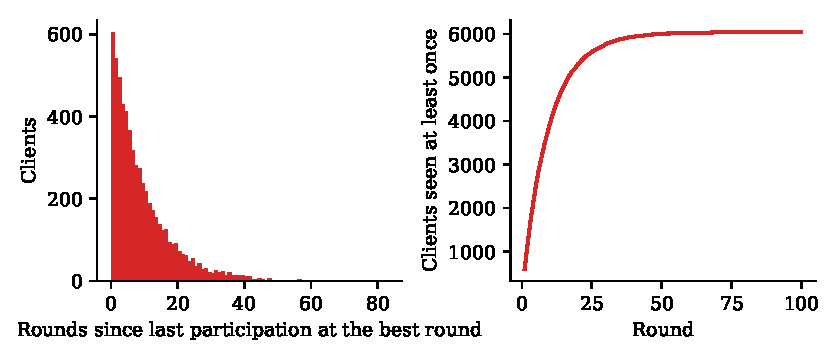
\includegraphics[width=\linewidth]{figures/fig_staleness.pdf}
  \caption{Left: rounds since the last participation of each client at the best round of the
  PFedRec run (\RunPfedrecShort). Right: cumulative number of distinct clients that have
  participated at least once, by round.}
  \label{fig:staleness}
\end{figure}

\section{Statistical Analysis}
\label{sec:setup-stats}

Every comparison between two scoring conditions on the same model, or between two methods, is a
paired comparison over users: $d_u = m_u^{A} - m_u^{B}$ for the per-user metric $m$. The
registered procedure, implemented once and reused for every experiment, reports:
\begin{itemize}[leftmargin=2em]
  \item the mean difference with a 95\% bootstrap confidence interval (10\,000 resamples,
        seed \Seed) \cite{efron1993bootstrap};
  \item the Wilcoxon signed-rank test \cite{wilcoxon1945} with the one-sided hypothesis
        registered for the experiment as primary, the two-sided $p$ as a check, and the
        rank-biserial correlation $r = (W^+ - W^-)/(W^+ + W^-)$ as effect size;
  \item zero differences handled by discarding them (the standard \code{wilcox} rule) in the
        primary test and by Pratt's rule \cite{pratt1959} as a registered sensitivity check,
        because in these experiments most users have $d_u = 0$ exactly;
  \item Holm's correction \cite{holm1979} across the cells of one experiment.
\end{itemize}
The tests describe variability across users for one trained model; they do not describe
variability across random seeds. When the mean and the rank test disagree, as happens when a
few users lose everything while many gain a little, both are reported and the mechanism is
stated (Section~\ref{sec:res-pfedrec}). \pending{paired tests across the four methods require
per-user scores for the Baseline, Personalized and Adaptive runs, which need the re-scoring
adapters for those modules and the runs' saved parameters}.

\section{Pre-registration Practice}
\label{sec:setup-prereg}

From November 2026 every experiment whose number reaches this thesis was registered before it
was run: a README in the result directory fixes the inputs with their hashes, the protocol, the
grid, the statistics, the trust checks that abort the run, numeric predictions, and the rule by
which the result will be reported; a fill-only result file is completed after the run and the
README is not edited afterwards except in a dated changelog. Appendix~\ref{app:posttune}
reproduces the predictions of the post-tuning experiment and their outcome, including the one
that was refuted.

\section{Compute}
\label{sec:setup-compute}

Each federated run took between \RunPfedrecHours{} and \RunPersonalizedHours{} hours of
wall-clock time on one GPU (Table~\ref{tab:runs}). The offline re-scoring of one variant over
all \DsUsers{} users takes seconds on a CPU; the four-cell post-tuning experiment took
\PtElapsedSec{} s. All analysis in Chapters~\ref{ch:results} and~\ref{ch:discussion} is
therefore reproducible without a GPU from the committed result files.

% Chapter 5 -- Results
% Status: sections 5.1, 5.3, 5.4 and 5.7 have audited numbers; 5.2 partial; 5.5 partial;
% 5.6 pending (privacy measurements). Every number is a macro or an \input table.
\chapter{Results}
\label{ch:results}

\section{Main Comparison of the Four Placements}
\label{sec:res-main}

Table~\ref{tab:main} reports the full-population metrics of the four methods at their best
round, and Figure~\ref{fig:group-bars} the \ndcg{} by user group. Three observations carry
through the rest of the chapter.

\begin{table}[htbp]
  \caption{Main comparison on MovieLens 1M, $N=\NClients$, $C=\ParticipationC$, $R=\NRounds$,
  full-population scoring at the restored best round. $^{\ddagger}$Centralised BPR-MF with the
  same leave-one-out and 99-negative protocol but an untuned configuration ($d=\CentralBprDim$,
  \CentralBprEpochs{} epochs, \CentralBprNeg{} negative); the PFedRec paper reports
  \PublishedCentralMfNdcg{} for a tuned centralised MF, so ``federated beats centralised'' is not
  claimed.}
  \label{tab:main}
  \centering\small
  % AUTO-GENERATED by thesis/scripts/build_assets.py -- do not edit by hand.
% final_metrics.best of each run (6040 users, best-round restore); centralized from results/centralized
\begin{tabular}{lcrrrrrr}
\toprule
Method & Best round & NDCG@10 & Sparse & Medium & Dense & HR@10 & HR@10 sparse \\
\midrule
Baseline (all-global BPR-MF) & 83 & 0.1882 & 0.2469 & 0.1994 & 0.1629 & 0.3258 & 0.4005 \\
Personalized (split learning) & 33 & 0.2275 & 0.2726 & 0.2451 & 0.2009 & 0.4197 & 0.4920 \\
PFedRec (+ final calibration) & 83 & 0.3447 & 0.4270 & 0.3802 & 0.2935 & 0.6111 & 0.7058 \\
Adaptive (dual-level, $\alpha$ blend) & 83 & 0.2144 & 0.2355 & 0.2264 & 0.1989 & 0.3868 & 0.4091 \\
\midrule
PFedRec (no calibration) & 100 & 0.3352 & 0.4057 & 0.3710 & 0.2870 & 0.5924 & 0.6712 \\
Centralized BPR-MF$^{\ddagger}$ & -- & 0.3332 & -- & -- & -- & 0.5901 & -- \\
\bottomrule
\end{tabular}

\end{table}

\begin{figure}[htbp]
  \centering
  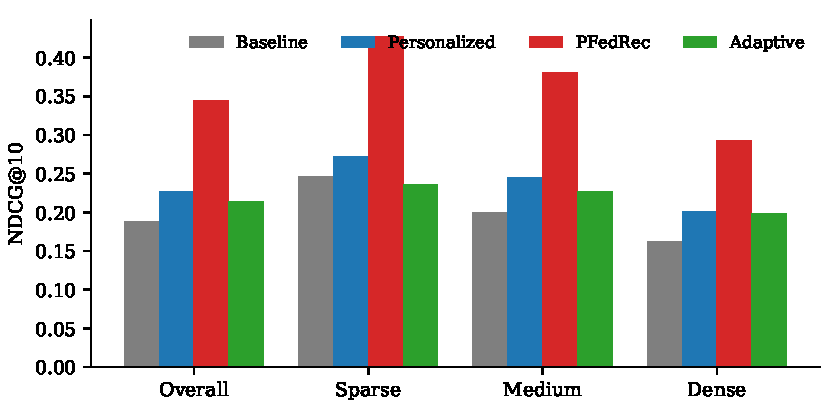
\includegraphics[width=0.9\linewidth]{figures/fig_group_bars.pdf}
  \caption{\ndcg{} of the four placements overall and by user group (best round, full
  population).}
  \label{fig:group-bars}
\end{figure}

First, keeping the user vector on the device is worth \GainPersonalizedVsBaselinePct\% \ndcg{}
over averaging it (\NdcgBaseline{} to \NdcgPersonalized) and
\GainPersonalizedVsBaselineSparsePct\% on sparse users, in the one pair of runs that differ in
nothing else (same loss, dimension, optimiser, learning rate, strategy and seed). Second, the
private head on a shared item table is far ahead of the three BPR-based placements
(\NdcgPfedrec{} against at most \NdcgPersonalized), and the ordering holds in every group. Third,
the adaptive blend is below the plain private user vector overall (\NdcgAdaptive{} against
\NdcgPersonalized) and, on the sparse group it was designed for, below even the all-global
baseline (\NdcgAdaptiveSparse{} against \NdcgBaselineSparse). The original hypothesis H1 is
refuted on this run.

\pending{paired per-user Wilcoxon tests with Holm correction and effect sizes for the six pairs
of methods, overall and by group; requires per-user scores of the Baseline, Personalized and
Adaptive runs (Section~\ref{sec:setup-stats}). Until then the differences in
Table~\ref{tab:main} are point estimates from one seed}.

\section{Best Round versus Last Round}
\label{sec:res-last-round}

Table~\ref{tab:last-round} places the in-loop metric at the selected best round and at round
\NRounds{} next to the full-population number. The ordering of the methods is the same at round
\NRounds{} as at the best round. The Personalized run peaks early (round
\RunPersonalizedBestRound) and its in-loop metric at round \NRounds{} is below its peak, while
the other three peak at round 83 and are close to their last-round value.

\begin{table}[htbp]
  \caption{Best-round and last-round \ndcg. In-loop columns are computed on the
  \ClientsPerRound{} clients sampled in that round; the full-population column at round \NRounds{}
  requires a re-score from the round-\NRounds{} checkpoint.}
  \label{tab:last-round}
  \centering\scriptsize
  % AUTO-GENERATED by thesis/scripts/build_assets.py -- do not edit by hand.
% eval_metrics_history (in-loop, sampled clients) vs final_metrics.best; full-pop round-100 column pending
\begin{tabular}{lrrrrr}
\toprule
Method & Best round & NDCG@10 best (6040 users) & In-loop NDCG@10 at best round (604) & In-loop NDCG@10 at round 100 (604) & Full-population NDCG@10 at round 100 \\
\midrule
Baseline (all-global BPR-MF) & 83 & 0.1882 & 0.2112 & 0.1556 & \pending{round-100 re-score} \\
Personalized (split learning) & 33 & 0.2275 & 0.2572 & 0.2482 & \pending{round-100 re-score} \\
PFedRec (+ final calibration) & 83 & 0.3447 & 0.3562 & 0.3436 & \pending{round-100 re-score} \\
Adaptive (dual-level, $\alpha$ blend) & 83 & 0.2144 & 0.2362 & 0.2342 & \pending{round-100 re-score} \\
\bottomrule
\end{tabular}

\end{table}

\begin{figure}[htbp]
  \centering
  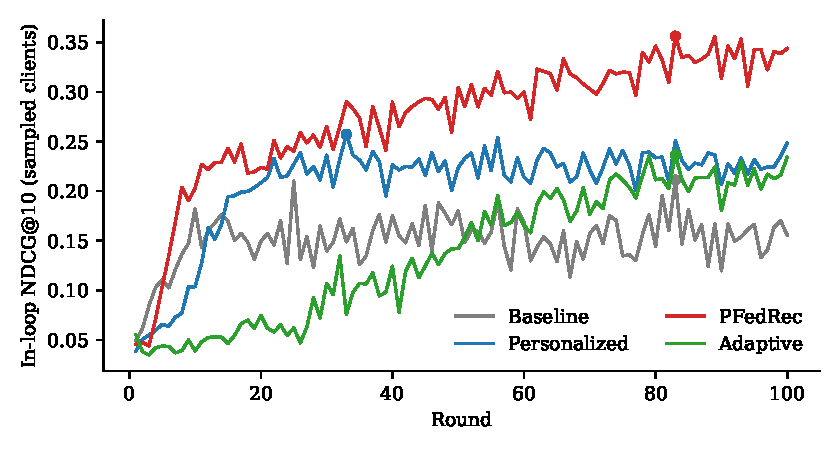
\includegraphics[width=0.9\linewidth]{figures/fig_training_curves.pdf}
  \caption{In-loop \ndcg{} of the sampled clients per round; the marker is the selected best
  round of each run.}
  \label{fig:training-curves}
\end{figure}

\section{Where Does the Value of Personalisation Live? Counterfactual Heads}
\label{sec:res-placement}

Table~\ref{tab:head-counterfactuals} and Figure~\ref{fig:head-counterfactuals} re-score the
PFedRec run with the item table, the bias and the 100 candidates per user held fixed and only
the head replaced (Section~\ref{sec:method-reeval}).

\begin{table}[htbp]
  \caption{Counterfactual heads on the PFedRec run \RunPfedrecShort. Every row scores the same
  item table and the same candidates; only the head differs. The blend row uses the
  hierarchical-conditional $\alpha_u$ rule of the adaptive method (mean $\alpha_u=\HeadAlphaMean$,
  range \HeadAlphaMin--\HeadAlphaMax).}
  \label{tab:head-counterfactuals}
  \centering\small
  % AUTO-GENERATED by thesis/scripts/build_assets.py -- do not edit by hand.
% reeval_<variant>_best.json of run cf72e0; same globals, same 100 candidates per user
\begin{tabular}{lrrrrrr}
\toprule
Head used at scoring time & NDCG@10 & $\Delta$ vs.\ own head & Sparse & Medium & Dense & HR@10 \\
\midrule
Own calibrated head $w_u$ (reference) & 0.3447 & -- & 0.4270 & 0.3802 & 0.2935 & 0.6111 \\
Blend $\alpha_u w_u + (1-\alpha_u)\bar w$, hierarchical-conditional $\alpha_u$ & 0.3061 & -0.0386 & 0.3483 & 0.3188 & 0.2842 & 0.5545 \\
Population-mean head $\bar w$ (uniform mean of 6040 heads) & 0.2510 & -0.0937 & 0.3113 & 0.2678 & 0.2208 & 0.4518 \\
Population head, weighted by interaction count & 0.2375 & -0.1072 & 0.2874 & 0.2550 & 0.2097 & 0.4373 \\
Another user's head (random permutation) & 0.1973 & -0.1474 & 0.2476 & 0.2126 & 0.1711 & 0.3727 \\
Freshly initialised head per user & 0.0741 & -0.2706 & 0.0725 & 0.0808 & 0.0692 & 0.1522 \\
One shared freshly initialised head & 0.0150 & -0.3297 & 0.0070 & 0.0135 & 0.0184 & 0.0291 \\
\bottomrule
\end{tabular}

\end{table}

\begin{figure}[htbp]
  \centering
  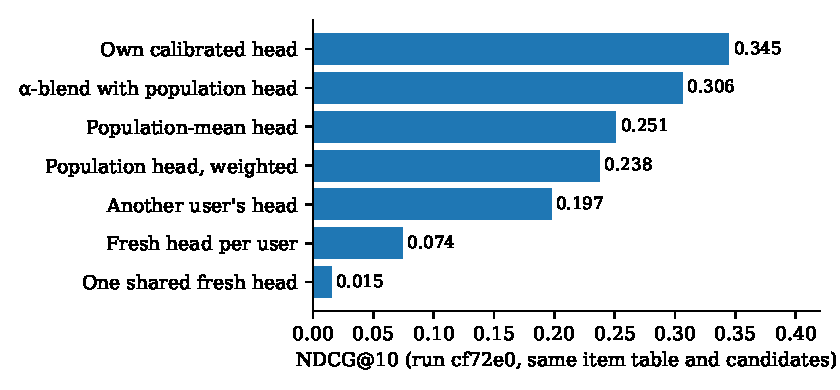
\includegraphics[width=0.85\linewidth]{figures/fig_head_counterfactuals.pdf}
  \caption{\ndcg{} of the counterfactual heads on the PFedRec run.}
  \label{fig:head-counterfactuals}
\end{figure}

The private head is load-bearing: the population-mean head costs \AbsDeltaHeadGlobalHead{}
\ndcg{} overall and the loss is largest in the sparse group (\NdcgPfedrecSparse{} to
\NdcgHeadGlobalHeadSparse), the group a population head is supposed to help. Another user's
head is worse still (\NdcgHeadShuffled), so the heads are personal and not merely a shared
offset. Blending does not help: the best single $\alpha$ on the grid is
$\alpha^\star=\HeadAlphaStarGlobal$ (the own head), and the data-driven rule of the adaptive
method, applied to this head, gives \NdcgHeadAlphaPolicyHc{} (\DeltaHeadAlphaPolicyHc), again
with the largest loss on sparse users (\NdcgHeadAlphaPolicyHcSparse). Hypothesis H3 holds on
this run. The two ``fresh head'' rows reproduce the cold-evaluation error of
Section~\ref{sec:setup-validity}: a freshly initialised head per user gives \NdcgHeadRandom{}
and one shared fresh head \NdcgHeadGlobalHeadCold, which is why a cold evaluation looks like a
broken model rather than like a crash. \pending{paired Wilcoxon tests of each row against the
own-head reference; the per-user scores of all rows are committed}.

\section{PFedRec: the Reproduction Gap and Post-tuning}
\label{sec:res-pfedrec}

The PFedRec paper reports \PublishedPfedrecNdcg{} \ndcg{} and \PublishedPfedrecHr{} \hr{} on
ML-1M; the reproduction under the thesis protocol gives \NdcgPfedrec{} and \HrPfedrec. The
official code run on the same machine and data gives \OfficialCodeNdcg{} and \OfficialCodeHr{}
(\pending{confirm the participation fraction, rounds and local epochs of that run}), so the gap
is not a machine or data artefact. Two protocol causes were put forward: the participation
fraction ($C=\ParticipationC$ here, $C=1$ in the paper) and the inference protocol (the official
code scores with a client-side post-tuned item table). The second cause was measured with the
registered experiment of Section~\ref{sec:method-posttune}.

\begin{table}[htbp]
  \caption{The three registered PFedRec rows (posttune README, rule fixed before the run) and
  the run without final calibration. Post-tuning rows use $E=1$, the official default; the
  $E=3$ cells are in Appendix~\ref{app:posttune}.}
  \label{tab:pfedrec-rows}
  \centering\small
  % AUTO-GENERATED by thesis/scripts/build_assets.py -- do not edit by hand.
% posttune/reeval_qu_diag_best.json baseline_metrics + metrics_by_cell (E=1 cells); ef41ab final_metrics.best
\begin{tabular}{lrrrrrr}
\toprule
Scoring protocol & NDCG@10 & Sparse & Medium & Dense & HR@10 & MRR \\
\midrule
PFedRec, scored with the shared item table (thesis number) & 0.3447 & 0.4270 & 0.3802 & 0.2935 & 0.6111 & 0.2821 \\
PFedRec, post-tuning, clean negatives ($E=1$) & 0.3181 & 0.4165 & 0.3611 & 0.2564 & 0.5584 & 0.2608 \\
PFedRec, post-tuning, official-code negatives ($E=1$) & 0.3789 & 0.4305 & 0.3891 & 0.3564 & 0.6642 & 0.3090 \\
\midrule
PFedRec without final calibration (run ef41ab, best round 100) & 0.3352 & 0.4057 & 0.3710 & 0.2870 & 0.5924 & -- \\
\bottomrule
\end{tabular}

\end{table}

Table~\ref{tab:pfedrec-rows} gives the registered three-row report. With clean negatives,
post-tuning \emph{lowers} \ndcg{} from \NdcgPfedrec{} to \NdcgEOneClean; with the official-code
negatives, which exclude the held-out test item, it \emph{raises} it to \NdcgEOneLeaky. The
paired statistics are in Table~\ref{tab:posttune-wilcoxon}, the per-group values in
Appendix~\ref{app:posttune}.

\begin{table}[htbp]
  \caption{Paired Wilcoxon tests of each post-tuning cell against the shared-table reference
  (\DsUsers{} users). $p$ one-sided tests the registered hypothesis ``cell $>$ reference'' with
  zero differences discarded; $p$ Pratt keeps them. Rows marked W$^-$=0 have no user whose score
  decreased, so their $p$-values follow from the construction (Section~\ref{sec:method-posttune})
  and the evidence is the confidence interval.}
  \label{tab:posttune-wilcoxon}
  \centering\scriptsize
  % AUTO-GENERATED by thesis/scripts/build_assets.py -- do not edit by hand.
% stats_wilcoxon.json cells.<cell>.by_scope.overall; n+/n-/n0 recomputed from the two per-user CSVs; W^-=0 marks p-values fixed by construction (< 1e-10); delta HR in the per-group table
\begin{tabular}{lrrrrrr}
\toprule
Cell & $\Delta$NDCG@10 [95\% CI] & $n_+/n_-/n_0$ & $p$ one-sided & $p$ two-sided & $p$ Pratt & $r$ \\
\midrule
$E=1$, clean & \mbox{-0.0266} \mbox{[-0.0315, -0.0217]} & 979/516/4545 & 1.0 & $9.5\times10^{-4}$ & $<10^{-10}$ & -0.099 \\
$E=1$, official-code & +0.0342 \mbox{[+0.0318, +0.0366]} & 1329/0/4711 & W$^-$=0 & W$^-$=0 & W$^-$=0 & +1.000 \\
$E=3$, clean & \mbox{-0.0685} \mbox{[-0.0757, -0.0613]} & 1281/1160/3599 & 1.0 & $<10^{-10}$ & 0.996 & -0.359 \\
$E=3$, official-code & +0.1073 \mbox{[+0.1026, +0.1122]} & 2502/0/3538 & W$^-$=0 & W$^-$=0 & W$^-$=0 & +1.000 \\
\bottomrule
\end{tabular}

\end{table}

\paragraph{Mechanism.} The candidates are items the user never interacted with, so their rows
in $\Qu$ change only when they are drawn as training negatives, and then they are pushed down.
With clean negatives the test item is drawn like any other candidate; when it is, the user's
test item falls out of the top 10 and that user's \ndcg{} becomes exactly $0$. At $E=1$ this
happened to \PtZeroLosersEOneClean{} users, all of whom have \ndcg{} $=0$ and a touched test
row, while \PtNPosEOneClean{} users gained a little because some of their 99 negatives were
pushed down. The mean therefore falls (\PtDeltaEOneClean, CI \PtCiEOneClean) while the rank
test under Pratt's rule, which weighs the many small gains, points the other way
(\PtPPrattEOneClean); the registered one-sided test (\PtPOneEOneClean) and the two-sided test
(\PtPTwoEOneClean) agree with the mean. Both are reported; the thesis uses the mean with the
mechanism stated. \decision{whether the thesis criterion for ``clean post-tuning hurts'' is the
mean with CI, or the rank test; recommendation: report both, conclude on the mean}.

With the official-code negatives the test item is never drawn, so no user can lose
($n_-=\PtNNegEOneLeaky$) and every touched candidate helps. Figure~\ref{fig:posttune-delta}
shows the two per-user distributions.

\begin{figure}[htbp]
  \centering
  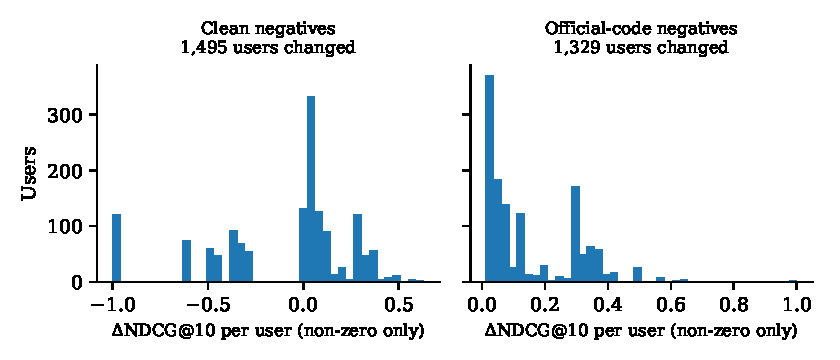
\includegraphics[width=0.9\linewidth]{figures/fig_posttune_delta.pdf}
  \caption{Per-user change of \ndcg{} after one post-tuning epoch, clean negatives (left) and
  official-code negatives (right); users with no change omitted.}
  \label{fig:posttune-delta}
\end{figure}

\paragraph{The size of the leak.} The two trajectories of a user differ only in the draws that
hit the test item, so the contrast official $-$ clean is non-zero for exactly
\PtContrastEOneNonZero{} users at $E=1$ and \PtContrastEThreeNonZero{} at $E=3$
(Table~\ref{tab:posttune-contrasts}). The overall difference of \PtContrastEOne{} \ndcg{}
(CI \PtContrastEOneCi) is therefore an average of about \PtContrastEOnePerUser{} \ndcg{} per
affected user: drawing the test item once as a negative is enough to remove it from the top 10.
The effect is concentrated in dense users (\PtContrastEOneDense{} against
\PtContrastEOneSparse{} for sparse users), who have more interactions and therefore more draws.

\begin{table}[htbp]
  \caption{Contrast between the official-code and the clean negative pool at the same number of
  post-tuning epochs; $n_{\neq 0}$ is the number of users whose two trajectories differ.}
  \label{tab:posttune-contrasts}
  \centering\small
  % AUTO-GENERATED by thesis/scripts/build_assets.py -- do not edit by hand.
% stats_wilcoxon.json contrasts.<A>__minus__<B>.by_scope; n_neq0 from the per-user CSV
\begin{tabular}{llrrrr}
\toprule
Contrast & Group & $\Delta$NDCG@10 (official $-$ clean) & 95\% CI & $p$ one-sided & $n_{\neq 0}$ \\
\midrule
$E=1$ & overall & +0.0608 & \mbox{[+0.0558, +0.0658]} & W$^-$=0 & 639 \\
$E=1$ & sparse & +0.0141 & \mbox{[+0.0078, +0.0213]} & $2.8\times10^{-5}$ & 21 \\
$E=1$ & medium & +0.0281 & \mbox{[+0.0225, +0.0338]} & W$^-$=0 & 108 \\
$E=1$ & dense & +0.1000 & \mbox{[+0.0913, +0.1090]} & W$^-$=0 & 510 \\
\midrule
$E=3$ & overall & +0.1758 & \mbox{[+0.1677, +0.1838]} & W$^-$=0 & 1,694 \\
$E=3$ & sparse & +0.0404 & \mbox{[+0.0295, +0.0524]} & $<10^{-10}$ & 55 \\
$E=3$ & medium & +0.0781 & \mbox{[+0.0692, +0.0875]} & W$^-$=0 & 295 \\
$E=3$ & dense & +0.2915 & \mbox{[+0.2780, +0.3046]} & W$^-$=0 & 1,344 \\
\bottomrule
\end{tabular}

\end{table}

\paragraph{Consequence for the limitation statement.} The registered rule selected the
sentence: \emph{part of the gap to the published number comes from the official code excluding
the test item from the training negatives during post-tuning}. Post-tuning itself, with clean
negatives, does not close the gap; it widens it. The row with the official-code negatives
(\NdcgEOneLeaky) is still \GapLeakyEOneToPublished{} below the published number, a residue
not separated between $C$ and the deviations K1--K3 of
Table~\ref{tab:posttune-deviations}. The $E=3$ cell with official-code negatives reaches
\NdcgEThreeLeaky, above the published \PublishedPfedrecNdcg{} already at $C=\ParticipationC$;
it refuted prediction A5 and is reported only as a diagnostic of the protocol, not as a result
of the method. \decision{cite the $E=3$ official-code cell in the appendix and limitations only
(recommended) or omit it}.

\section{The Adaptive Method as a Negative Result}
\label{sec:res-adaptive}

The adaptive method ranks third overall and last on sparse users (Table~\ref{tab:main}). Three
causes were identified; two are measured here and one in Section~\ref{sec:res-privacy}.

\paragraph{The blending weight pulls taste toward the mean.} The counterfactual of
Section~\ref{sec:res-placement} applies the same hierarchical-conditional rule to the PFedRec
head and loses \AbsDeltaHeadAlphaPolicyHc{} \ndcg{}, most on sparse users, where the rule assigns
the lowest $\alpha_u$ (mean $\alpha_u = \HeadAlphaMean$ overall). On the grid, the best single
weight is the fully local one. This is indirect evidence, measured on the PFedRec head rather
than on the adaptive run's user vector; \pending{direct measurement on the adaptive run: the
distance of the blended vector $\tilde{\vect{p}}_u$ to the prototype and to $\pu$ by group, and
a re-score with $\alpha_u=1$ (no blend) from the run's cached state}.

\paragraph{The per-user network is too large for the data.} The PersonalMLP has
\ParamsPersonalMlp{} private parameters per client, trained on a median of \DsMedianRatings{}
interactions and on at most \ExpectedParticipations{} participations in expectation, each of
one local epoch. \pending{parameters-per-interaction by group and, if time permits, a re-score
with the MLP branch zeroed from the cached state}.

\paragraph{Uploading the user vector weakens privacy.} Section~\ref{sec:res-privacy}.

\section{Privacy and Communication}
\label{sec:res-privacy}

Table~\ref{tab:params-comm} gives the parameters each placement aggregates, keeps private, and
uploads per participation, derived from the architectures. The private-head placement uploads
the least (\ParamsPfedrecGlobal{} parameters), the split-learning placements about twice as
much, and the all-global baseline \ParamsBaselineGlobal, including every user vector. The
adaptive method uploads the global part plus the \ParamsAdaptiveUploadExtra{} floats of $\pu$.

\begin{table}[htbp]
  \caption{Parameters per placement. $^{\dagger}$Counted from the architecture; the measured
  size of the Flower messages is pending.}
  \label{tab:params-comm}
  \centering\small
  % AUTO-GENERATED by thesis/scripts/build_assets.py -- do not edit by hand.
% derived from federated_config dims (users 6040, items 3706); measured byte counts are pending
\begin{tabular}{lrrr}
\toprule
Method & Global parameters (aggregated) & Local parameters per client & Uploaded per participating client per round$^{\dagger}$ \\
\midrule
Baseline (all-global BPR-MF) & 633,491 & 0 & 633,491 \\
Personalized (split learning) & 240,891 & 65 & 240,891 \\
PFedRec & 118,593 & 32 & 118,593 \\
Adaptive (dual-level) & 240,891 & 197,701 & 240,955 \\
\bottomrule
\end{tabular}

\end{table}

\pending{byte-level table measured from the actual Flower messages (upload and download per
client per round, per method)}.

\pending{preference-reconstruction attack on the adaptive run: for every user, top-10 of
$\pu^\top\Qtab^\top$ over all \DsItems{} items versus the user's interacted items; hits overall
and by group against the random and popularity baselines; one paragraph on secure aggregation
as the mitigation and on why it does not cover the $\pu$ upload}.

\section{The Cost of Stale Private Parts}
\label{sec:res-staleness}

At the best round of the PFedRec run the median client was \StaleMedian{} rounds stale and
\StaleOverTen\% of the clients more than ten rounds (Figure~\ref{fig:staleness}). The cited run
calibrates every head for one epoch against the restored item table before scoring; the
otherwise comparable run without calibration (\RunPfedrecNocalShort, best round
\RunPfedrecNocalBestRound) scores \NdcgPfedrecNocal, a difference of \DeltaPfedrecCalibration{}
that is confounded by the best round (\RunPfedrecBestRound{} against
\RunPfedrecNocalBestRound) and by the code version. \decision{how to measure the stale-head
cost: (i) per-user \ndcg{} of the calibrated run against rounds since last participation;
(ii) re-score the Personalized run before and after one calibration epoch, paired, which
measures the same phenomenon on the user vector; (iii) keep the confounded run pair with the
confounds stated. Recommendation: (i) and (ii), with (ii) as the main measurement if the run's
saved state is available}. \pending{the chosen measurement, pre-registered before it is run}.

% Chapter 6 -- Discussion
% Status: basic draft; revise after the pending results and the advisor's decisions.
\chapter{Discussion}
\label{ch:discussion}

\section{Assessment of the Hypotheses}
\label{sec:disc-hypotheses}

\begin{description}[leftmargin=3em, style=nextline]
  \item[H1 (original): refuted.] The adaptive method does not beat the other placements; it is
        below the private user vector overall and below every method on sparse users
        (Section~\ref{sec:res-main}). \pending{paired tests to state the margins with
        confidence intervals}.
  \item[H2: supported on the mean.] Keeping the user vector private improves \ndcg{} by
        \GainPersonalizedVsBaselinePct\% over averaging it, with everything else equal.
        \pending{paired test}.
  \item[H3: supported.] On the PFedRec model the population-mean head costs
        \DeltaHeadGlobalHead, no $\alpha$ on the grid beats $\alpha=1$, and the data-driven
        rule loses \AbsDeltaHeadAlphaPolicyHc{} (Section~\ref{sec:res-placement}).
  \item[H4: supported; prediction A5 refuted.] Clean post-tuning lowers \ndcg{}
        (\PtDeltaEOneClean, CI \PtCiEOneClean); official-code negatives raise it
        (\PtDeltaEOneLeaky); the contrast is \PtContrastEOne{} and is carried by
        \PtContrastEOneNonZero{} users. The $E=3$ official-code cell exceeded the registered
        ceiling of 0.394 and the published number itself (Section~\ref{sec:res-pfedrec}).
\end{description}

\section{Why Blending with Population Knowledge Did Not Help}
\label{sec:disc-adaptive}

Three mechanisms are consistent with the measurements. First, the population prototype is
nearly uninformative for ranking: the uniform mean of \DsUsers{} heads or vectors cancels
exactly the directions that distinguish one user from another, so any weight $(1-\alpha_u)>0$
on it moves the user toward a point that ranks items like a popularity list. The counterfactual
rows of Table~\ref{tab:head-counterfactuals} show this directly: the population head is worth
less than the own head in every group, and most in the sparse group. Second, the
hierarchical-conditional rule assigns the smallest $\alpha_u$ to exactly those users, so the
rule applies the strongest pull where the prototype is least adequate. Third, the data are not a
cold-start setting: a ``sparse'' MovieLens user still has at least 19 training interactions, enough
to fit a 64-dimensional vector or a 32-dimensional head, so there is little to gain from
borrowing. These observations are consistent with APFL's analysis, in which the optimal mixing
weight approaches the local model as the local and global optima diverge
\cite{deng2020apfl}, and with FedTHE's finding that test-time ensembling of a global and a local
head helps under distribution shift and little in-distribution \cite{jiang2023fedthe}. The
PersonalMLP adds a second problem: \ParamsPersonalMlp{} private parameters trained on a median
of \DsMedianRatings{} interactions in about \ExpectedParticipations{} short visits is a
capacity-to-data ratio under which a non-linear scorer cannot be expected to beat an inner
product. The adaptive design would need a different setting to be useful: a genuine cold-start
population, or a shift between a user's training and test behaviour.

\section{What Post-tuning Measures and What It Does Not}
\label{sec:disc-posttune}

The post-tuning experiment separates three things that the literature reports as one number.
(i) Post-tuning the item table on the client with honest negatives is a \emph{cost} under this
protocol: the client pushes down whatever it draws, and it cannot know that one of the items it
draws is the one the evaluation will ask for. (ii) Excluding the held-out item from the
negatives converts that cost into a gain, because the only rows that can then move among the
candidates are the 99 negatives, which can only move down. This is a property of the evaluation
protocol, not of the method, and it is invisible when the item table is shared, because the
update of one user is diluted among the \ClientsPerRound{} clients of a round. (iii) What
remains of the gap after (ii) is not separated between the participation fraction and the three
deviations K1--K3 of Table~\ref{tab:posttune-deviations}; the official code run on the same
machine (\OfficialCodeNdcg) bounds the sum of those effects if its configuration is confirmed
to be the official default (\pending{confirmation}). The thesis therefore reports PFedRec at
\NdcgPfedrec{} with the shared table as its number, lists the two post-tuning rows next to it,
and states the limitation with the measured cause. \decision{final wording of the limitation
paragraph: (A) two measured causes, $C$ unmeasured but bounded, and the negative-pool leak with
its size; or (B) keep ``no post-tuning at evaluation'' as the cause with a footnote giving the
measurement that has the opposite sign}.

A point on statistics. In the clean cells the mean and the rank test disagree
(Table~\ref{tab:posttune-wilcoxon}): under Pratt's treatment of ties the test almost reduces to
counting the users who gained a little (\PtNPosEOneClean) against those who lost everything
(\PtNNegEOneClean{} at $E=1$, every one of them to \ndcg{} $=0$), and it ignores the size of
the losses. Both views are legitimate answers to different questions; the thesis reports both
and concludes on the mean, because a recommender is judged on its average ranking quality and
a user whose test item disappears from the list is a worse outcome than many users whose item
moves up by one rank.

\section{Fairness of the Placement Comparison}
\label{sec:disc-fairness}

The four cited runs differ in more than the placement (Table~\ref{tab:asymmetries}). PFedRec
uses BCE with four negatives, SGD and $d=\DimPfedrec$; the three others use BPR, Adam and
$d=\DimMf$. Only PFedRec has a final calibration of its private part. The best rounds differ,
and all are selected on the test item. These asymmetries limit the comparison to the reading
``each method at its own, author-faithful configuration'': the placement study is clean only
within the BPR family (Baseline against Personalized), and the PFedRec margin should be read as
a design-level result rather than as a controlled effect of the head alone. \decision{(A) keep
the author-faithful configurations and present Table~\ref{tab:asymmetries} as the reading
guide, or (B) first calibrate the Personalized and Adaptive runs offline to remove the
calibration asymmetry}.

\begin{table}[htbp]
  \caption{Configuration asymmetries between the four cited runs.}
  \label{tab:asymmetries}
  \centering\small
  \fittable{% AUTO-GENERATED by thesis/scripts/build_assets.py -- do not edit by hand.
% configuration asymmetries between the four cited runs
\begin{tabular}{lllll}
\toprule
Aspect & Baseline & Personalized & PFedRec & Adaptive \\
\midrule
Loss & BPR & BPR & BCE (4 negatives) & BPR \\
Embedding dimension & 64 & 64 & 32 & 64 \\
Optimizer & Adam & Adam & SGD (alternating) & Adam \\
Strategy & fedavg & fedavg & fedavg & fedprox \\
Final calibration of the local part & n/a & no & yes (1 epoch, items frozen) & no \\
Best round (selected on the test item) & 83 & 33 & 83 & 83 \\
Extra upload beyond the global part & none & none & none & $p_u$ (prototype) \\
\bottomrule
\end{tabular}
}
\end{table}

\section{Implications for Practice}
\label{sec:disc-practice}

For a cross-device recommender at low participation the results suggest: keep the user-specific
part on the device (it is both the most private and the most accurate choice of the BPR family);
if the model allows it, place personalisation in a private scoring function on a shared item
table rather than in a user vector, and re-align that function to the current table before
serving; do not blend the private part with a population average unless the population is
cold; never upload the user vector; and treat any client-side fine-tuning of the item table at
inference as a protocol decision that must be reported with its negative-sampling rule.
Operationally, evaluate stateful clients with a cache-miss counter, a validity sidecar and a
replay gate, because the failure mode is silent.

\section{Threats to Validity}
\label{sec:disc-threats}

\paragraph{Internal.} One seed per run; no validation item, so best rounds are selected on the
test item (inflation of \InflationBaseline{} to \InflationPfedrec{} points,
Section~\ref{sec:setup-validity}); configuration asymmetries (Section~\ref{sec:disc-fairness});
the adaptive run kept a contrastive term enabled and was not calibrated; the centralised
comparator is untuned. The paired tests, where available, describe users, not seeds.

\paragraph{Construct.} Sampled metrics with 99 negatives are known to disagree with exhaustive
ones \cite{krichene2020sampled}; the comparison is valid because every method ranks the same
candidates, but the absolute numbers are protocol-specific. The ``sparse'' group of MovieLens 1M
is not a cold-start group.

\paragraph{External.} One dataset, one domain (films), one participation fraction. The leak
mechanism of Section~\ref{sec:disc-posttune} applies to any method that fine-tunes a per-user
item table at inference, but its size depends on the number of interactions per user and on
the number of epochs.

\paragraph{Measurement.} All full-population numbers come from runs classified as valid, with
cache-miss counters where the code recorded them; the offline tool reproduced the PFedRec
evaluation bit-exactly. Numbers in this document are generated from the result files by one
script and are not typed by hand.

% Chapter 7 -- Conclusion and Future Work
% Status: basic draft.
\chapter{Conclusion and Future Work}
\label{ch:conclusion}

\section{Conclusion}
\label{sec:conc-conclusion}

This thesis asked where personalisation should live in a cross-device federated recommender,
what each placement costs in privacy, and how stateful clients must be evaluated. Under one
locked protocol on MovieLens 1M (\NClients{} clients, $C=\ParticipationC$, \NRounds{} rounds,
shared candidate lists), the placement of the personal part dominated every other design
choice. Keeping the user vector on the device improved \ndcg{} by
\GainPersonalizedVsBaselinePct\% over averaging it with nothing else changed; a private scoring
head on a shared item table reached \NdcgPfedrec, and on that model the private head was worth
\DeltaHeadGlobalHead{} against the population head, with no blend between the two recovering
the loss. The thesis's own adaptive method, which blends the user vector with a population
prototype and adds a per-user neural scorer, was reported as a negative result with three
measured or identified causes: the blend pulls taste toward the mean where the prototype is
least adequate, the private network is oversized for the data, and the upload of the user vector
opens a leakage channel that the other placements do not have.

The comparison with the published PFedRec number was treated as a measurement problem. A
pre-registered re-score showed that client-side post-tuning of the item table lowers \ndcg{}
under honest negative sampling and raises it only when the held-out item is excluded from the
negatives as in the released code, a difference of \PtContrastEOne{} carried entirely by the
\PtContrastEOneNonZero{} users whose test item was drawn. The thesis reports its number with
the shared item table and states the measured cause in its limitations. Finally, the work
established the safeguards without which none of these numbers could be trusted: a
cold-evaluation error that reduced \ndcg{} \ColdEvalRatio-fold was found and fixed, cache-miss
counters and validity sidecars were added to every run, and an offline re-scoring tool that
reproduces the federated evaluation exactly became the basis of every analysis.
\pending{one sentence on the privacy measurements and the stale-head cost once they are in}.

\section{Future Work}
\label{sec:conc-future}

\begin{itemize}[leftmargin=2em]
  \item \textbf{Private item table with row-wise blending.} A client-held item table
        $\Qu$ that is blended with the global table only on the rows of items the user
        interacted with was proposed during this work and withdrawn after analysis: the private
        part would then live only on items the user has already seen and could not reach the
        items to be recommended. A formulation that propagates the private adjustment to
        unseen items (for example through item--item similarity) remains open, and its
        evaluation must use the clean negative pool of Section~\ref{sec:method-posttune}.
  \item \textbf{Secure aggregation and a measured privacy budget.} The item-table update
        pattern is the leakage channel common to all placements; implementing secure
        aggregation \cite{bonawitz2017secagg} in the framework and measuring what the server
        can still infer would close the gap between the threat model and the deployment.
  \item \textbf{Seeds and a validation item.} Two further seeds for the three close cells and a
        protocol with a validation item would turn the single-seed point estimates into
        intervals and remove the best-round inflation.
  \item \textbf{Participation fraction.} A PFedRec run at $C=1$ under the thesis protocol
        would separate the share of the reproduction gap due to participation from the share
        due to the deviations K1--K3.
  \item \textbf{A cold-start population.} The adaptive design should be re-evaluated where its
        assumptions hold, on a dataset with genuinely cold users or with a train/test shift per
        user, before it is abandoned.
\end{itemize}


% ---------------------------------------------------------------------------
% References
% ---------------------------------------------------------------------------
\cleardoublepage
\printbibliography[heading=bibintoc, title={References}]

% ---------------------------------------------------------------------------
% Appendices
% ---------------------------------------------------------------------------
\cleardoublepage
\appendix
\renewcommand{\chaptertitlename}{Appendix}
\addtocontents{toc}{\protect\vspace{0.8em}\protect\noindent\protect\textbf{Appendices}\protect\par}
% Appendix A -- full tables of the post-tuning re-score (registered experiment).
\chapter{Post-tuning Re-score of PFedRec: Full Tables}
\label{app:posttune}

The experiment is described in Section~\ref{sec:method-posttune} and its pre-registration is the
file \path{posttune/README.md} in the directory of run \RunPfedrecShort{} under
\path{results/federated/pfedrec/} (version 1.1, 4 November 2026); the filled result file is
\path{RESULT.md} in the same directory. Inputs: the restored
best-round item table (SHA-256 \PtGlobalsSha), the \DsUsers{} calibrated heads, and the
candidate lists of the run's own evaluation. The run took \PtElapsedSec{} s on a CPU for the
four cells. Trust checks: the replay of the reference matched the run bit-exactly; no
non-finite value in any $\Qu$; untouched rows bit-identical to $\Qtab$ on a sample of users;
the test item was drawn at least once for \PtNHitClean{} users in the clean pool and for
\PtNHitLeaky{} in the official-code pool; and no user's score decreased in the official-code
cells (the registered monotonicity check). The median row shift was \PtRowShiftMedianEOne{} at
$E=1$ and \PtRowShiftMedianEThree{} at $E=3$ against a median row norm of \PtRowNormMedian{} in
$\Qtab$.

\section{All Four Cells}

\begin{table}[htbp]
  \caption{\ndcg{} / \hr{} / \mrr{} of the reference and the four cells, overall and by group.}
  \label{tab:posttune-cells}
  \centering\scriptsize
  \fittable{% AUTO-GENERATED by thesis/scripts/build_assets.py -- do not edit by hand.
% posttune/reeval_qu_diag_best.json: one row per cell and metric, columns = overall and groups
\begin{tabular}{llrrrr}
\toprule
Cell & Metric & Overall & Sparse & Medium & Dense \\
\midrule
Shared item table (reference) & NDCG@10 & 0.3447 & 0.4270 & 0.3802 & 0.2935 \\
 & HR@10 & 0.6111 & 0.7058 & 0.6688 & 0.5387 \\
 & MRR & 0.2821 & 0.3552 & 0.3083 & 0.2409 \\
\midrule
$E=1$, clean & NDCG@10 & 0.3181 & 0.4165 & 0.3611 & 0.2564 \\
 & HR@10 & 0.5584 & 0.6848 & 0.6326 & 0.4641 \\
 & MRR & 0.2608 & 0.3474 & 0.2937 & 0.2105 \\
\midrule
$E=1$, official-code & NDCG@10 & 0.3789 & 0.4305 & 0.3891 & 0.3564 \\
 & HR@10 & 0.6642 & 0.7108 & 0.6792 & 0.6394 \\
 & MRR & 0.3090 & 0.3583 & 0.3165 & 0.2893 \\
\midrule
$E=3$, clean & NDCG@10 & 0.2762 & 0.3981 & 0.3347 & 0.1956 \\
 & HR@10 & 0.4704 & 0.6539 & 0.5792 & 0.3324 \\
 & MRR & 0.2305 & 0.3329 & 0.2742 & 0.1672 \\
\midrule
$E=3$, official-code & NDCG@10 & 0.4520 & 0.4385 & 0.4128 & 0.4871 \\
 & HR@10 & 0.7505 & 0.7219 & 0.7063 & 0.7937 \\
 & MRR & 0.3738 & 0.3649 & 0.3381 & 0.4047 \\
\bottomrule
\end{tabular}
}
\end{table}

\section{Per-group Paired Tests}

\begin{table}[htbp]
  \caption{Paired tests against the shared-table reference by user group. Where $n_-=0$ the
  one-sided $p$ follows from the construction; for groups with few changed users the computed
  value is printed.}
  \label{tab:posttune-groups}
  \centering\scriptsize
  \fittable{% AUTO-GENERATED by thesis/scripts/build_assets.py -- do not edit by hand.
% stats_wilcoxon.json cells.<cell>.by_scope.<group>; structural label when W^-=0 and >60 users changed
\begin{tabular}{llrrrrrr}
\toprule
Cell & Group & $\Delta$NDCG@10 & 95\% CI & $\Delta$HR@10 & $p$ one-sided & $p$ Pratt & $n_+/n_-/n_0$ \\
\midrule
$E=1$, clean & sparse & \mbox{-0.0105} & \mbox{[-0.0181, -0.0039]} & \mbox{-0.0210} & 0.955 & 0.124 & 30/21/758 \\
$E=1$, clean & medium & \mbox{-0.0191} & \mbox{[-0.0250, -0.0133]} & \mbox{-0.0362} & 0.64 & $<10^{-10}$ & 246/108/1968 \\
$E=1$, clean & dense & \mbox{-0.0371} & \mbox{[-0.0460, -0.0286]} & \mbox{-0.0746} & 0.999 & $<10^{-10}$ & 703/387/1819 \\
\midrule
$E=1$, official-code & sparse & +0.0036 & \mbox{[+0.0018, +0.0058]} & +0.0049 & $2.6\times10^{-7}$ & $4.6\times10^{-9}$ & 33/0/776 \\
$E=1$, official-code & medium & +0.0090 & \mbox{[+0.0073, +0.0108]} & +0.0103 & W$^-$=0 & W$^-$=0 & 262/0/2060 \\
$E=1$, official-code & dense & +0.0629 & \mbox{[+0.0583, +0.0675]} & +0.1007 & W$^-$=0 & W$^-$=0 & 1034/0/1875 \\
\midrule
$E=3$, clean & sparse & \mbox{-0.0289} & \mbox{[-0.0414, -0.0176]} & \mbox{-0.0519} & 0.971 & 0.00418 & 91/53/665 \\
$E=3$, clean & medium & \mbox{-0.0454} & \mbox{[-0.0550, -0.0363]} & \mbox{-0.0896} & 1.0 & $9.3\times10^{-9}$ & 507/279/1536 \\
$E=3$, clean & dense & \mbox{-0.0979} & \mbox{[-0.1099, -0.0858]} & \mbox{-0.2063} & 1.0 & 1.0 & 683/828/1398 \\
\midrule
$E=3$, official-code & sparse & +0.0115 & \mbox{[+0.0081, +0.0152]} & +0.0161 & W$^-$=0 & W$^-$=0 & 98/0/711 \\
$E=3$, official-code & medium & +0.0326 & \mbox{[+0.0294, +0.0361]} & +0.0375 & W$^-$=0 & W$^-$=0 & 629/0/1693 \\
$E=3$, official-code & dense & +0.1936 & \mbox{[+0.1850, +0.2020]} & +0.2551 & W$^-$=0 & W$^-$=0 & 1775/0/1134 \\
\bottomrule
\end{tabular}
}
\end{table}

\section{Registered Predictions and Outcome}

\begin{table}[htbp]
  \caption{The five predictions registered before the run and their outcome. A1 was judged on
  the mean with its confidence interval; under Pratt's treatment of ties the rank test points
  the other way (Section~\ref{sec:res-pfedrec}).}
  \label{tab:predictions}
  \centering\small
  \fittable{% AUTO-GENERATED by thesis/scripts/build_assets.py -- do not edit by hand.
% posttune/README.md section 8 predictions vs RESULT.md section 4 (numbers via macros)
\begin{tabular}{@{}p{0.04\linewidth}>{\raggedright\arraybackslash}p{0.40\linewidth}>{\raggedright\arraybackslash}p{0.36\linewidth}>{\raggedright\arraybackslash}p{0.13\linewidth}@{}}
\toprule
\# & Prediction (registered before the run) & Observed & Verdict \\
\midrule
A1 & Clean negatives, $E=1$: NDCG@10 below the reference; $E=3$ below $E=1$ & \NdcgEOneClean{} ($\Delta$ \PtDeltaEOneClean{}, CI \PtCiEOneClean{}); $E=3$: \NdcgEThreeClean{} & Correct on the mean \\
A2 & Official-code negatives, $E=1$: $\Delta \geq +0.010$, one-sided $p<0.05$; $E=3 \geq E=1$ & $\Delta$ \PtDeltaEOneLeaky{} \PtCiEOneLeaky{}; $E=3$: \NdcgEThreeLeaky{} & Correct \\
A3 & Official $-$ clean $\geq +0.010$ at both $E$ & \PtContrastEOne{} and \PtContrastEThree{} & Correct \\
A4 & Dense users have the largest $|\Delta|$ in all four cells & holds in 4/4 cells (Table~\ref{tab:posttune-groups}) & Correct \\
A5 & No cell reaches 0.394 (half of the gap to the published 0.4436) & $E=3$, official-code negatives: \NdcgEThreeLeaky{} & Refuted \\
\bottomrule
\end{tabular}
}
\end{table}

\section{Reporting Rule}

The README fixed, before the run, that the thesis table would contain three rows (reference;
clean $E=1$; official-code $E=1$) with no selection of the highest cell, that the $E=3$ cells
would appear only in this appendix, and that the limitation sentence would be chosen by the
following rule: if official $-$ clean at $E=1$ is at least $+0.010$ with one-sided $p<0.05$,
then ``part of the gap to the published number comes from the official code excluding the test
item from the negatives during post-tuning''; otherwise ``the difference in the negative pool is
negligible and the residual gap is not separated between $C$ and K1--K3''. The first branch
applied (\PtContrastEOne, CI \PtContrastEOneCi).

% Appendix B -- configurations of the cited runs and per-group metrics.
\chapter{Configurations and Per-group Metrics}
\label{app:config}

\begin{table}[htbp]
  \caption{Configuration of the four cited runs, read from the \code{federated\_config} block of
  each \code{results.json}. Values that the BPR-based modules take from the shared mode profile
  (local epochs, optimiser, loss, training negatives) are included.}
  \label{tab:hyperparams}
  \centering\small
  \fittable{% AUTO-GENERATED by thesis/scripts/build_assets.py -- do not edit by hand.
% federated_config of each cited run (results.json)
\begin{tabular}{lllll}
\toprule
Setting & Baseline & Personalized & PFedRec & Adaptive \\
\midrule
Strategy & fedavg & fedavg & fedavg & fedprox \\
Model type & bpr & bpr & -- & dual \\
Embedding dim & 64 & 64 & -- & 64 \\
Latent dim & -- & -- & 32 & -- \\
Learning rate & 0.005 & 0.005 & -- & 0.005 \\
Learning rate (head) & -- & -- & 0.1 & -- \\
Item LR multiplier $\eta$ & -- & -- & 80.0 & -- \\
Local epochs & 1 & 1 & 1 & 1 \\
Training negatives & 4 & 4 & 4 & 4 \\
FedProx $\mu$ & 0.01 & 0.01 & -- & 0.01 \\
Dropout & 0.1 & 0.1 & -- & 0.1 \\
Participation $C$ & 0.1 & 0.1 & 0.1 & 0.1 \\
Rounds $R$ & 100 & 100 & 100 & 100 \\
Aggregation weights & num\_positives & num\_positives & uniform & num\_positives \\
Loss & bpr & bpr & bce & bpr \\
Optimizer & adam & adam & sgd & adam \\
Fusion & -- & -- & -- & concat \\
PersonalMLP hidden & -- & -- & -- & 512--256--128 \\
Prototype momentum & -- & -- & -- & 0.9 \\
Checkpoint rule & best\_round\_restore & best\_round\_restore & best\_round\_restore & best\_round\_restore \\
Seed & 42 & 42 & 42 & 42 \\
\bottomrule
\end{tabular}
}
\end{table}

\begin{table}[htbp]
  \caption{Full-population metrics of the four methods by user group at the best round.}
  \label{tab:main-groups}
  \centering\small
  \fittable{% AUTO-GENERATED by thesis/scripts/build_assets.py -- do not edit by hand.
% final_metrics.best per group; MRR only where the run logged it
\begin{tabular}{llrrrr}
\toprule
Method & Group & Users & NDCG@10 & HR@10 & MRR \\
\midrule
Baseline (all-global BPR-MF) & overall & 6,040 & 0.1882 & 0.3258 & -- \\
 & sparse & 809 & 0.2469 & 0.4005 & -- \\
 & medium & 2,322 & 0.1994 & 0.3407 & -- \\
 & dense & 2,909 & 0.1629 & 0.2932 & -- \\
\midrule
Personalized (split learning) & overall & 6,040 & 0.2275 & 0.4197 & -- \\
 & sparse & 809 & 0.2726 & 0.4920 & -- \\
 & medium & 2,322 & 0.2451 & 0.4531 & -- \\
 & dense & 2,909 & 0.2009 & 0.3730 & -- \\
\midrule
PFedRec (+ final calibration) & overall & 6,040 & 0.3447 & 0.6111 & -- \\
 & sparse & 809 & 0.4270 & 0.7058 & -- \\
 & medium & 2,322 & 0.3802 & 0.6688 & -- \\
 & dense & 2,909 & 0.2935 & 0.5387 & -- \\
\midrule
Adaptive (dual-level, $\alpha$ blend) & overall & 6,040 & 0.2144 & 0.3868 & -- \\
 & sparse & 809 & 0.2355 & 0.4091 & -- \\
 & medium & 2,322 & 0.2264 & 0.4065 & -- \\
 & dense & 2,909 & 0.1989 & 0.3647 & -- \\
\bottomrule
\end{tabular}
}
\end{table}

\section*{Adaptive $\alpha$ rule}
\label{app:alpha-rule}

\pending{the exact hierarchical-conditional rule as implemented (factor definitions,
normalisations, thresholds, penalties and the $[0.1, 0.95]$ clipping), copied from
\code{adaptive\_alpha.py}; and the distribution of $\alpha_u$ by group on the cited run}.

% Appendix C -- reproducibility record. Keep in sync with the repository.
\chapter{Reproducibility}
\label{app:repro}

\section{Repository and Result Files}

All code, result files and this document live in one repository:
\begin{itemize}[nosep]\raggedright
  \item \path{federated-baseline-cf}, \path{federated-personalized-cf}, \path{federated-pfedrec}
        and \path{federated-adaptive-personalized-cf}: the four federated methods;
  \item \path{scripts/foundation/fedrec_foundation}: the shared foundation library (data loading,
        partitioning, evaluation);
  \item \path{scripts/thesis/reeval.py} and \path{scripts/thesis/gate_stats.py}: the offline
        re-scoring tool and the paired statistics;
  \item \path{results/federated/<module>/<run_id>/}: one directory per cited run with
        \code{results.json}, \code{manifest.json} and \code{EVAL\_VALIDITY.json}; the PFedRec run
        also holds the per-user scores of every re-scoring variant
        (\path{reeval_*_best_per_user.csv}) and the \code{posttune/} directory with the
        registered experiment.
\end{itemize}

\begin{table}[htbp]
  \caption{Identifiers of the cited runs.}
  \label{tab:repro-runs}
  \centering\small
  \begin{tabular}{lll}
    \toprule
    Method & Run identifier & Code commit \\
    \midrule
    Baseline & \RunBaselineId & \RunBaselineCommit \\
    Personalized & \RunPersonalizedId & \RunPersonalizedCommit \\
    PFedRec (+ calibration) & \RunPfedrecId & \RunPfedrecCommit \\
    Adaptive & \RunAdaptiveId & \RunAdaptiveCommit \\
    \bottomrule
  \end{tabular}
\end{table}

\section{Regenerating the Tables and Figures}

The script \path{thesis/scripts/build_assets.py} produces every table, figure and number
macro in this document from the files above:
\begin{verbatim}
python thesis/scripts/build_assets.py   # tables, numbers, figures
cd thesis && latexmk -xelatex main.tex  # the PDF
\end{verbatim}
The script fails if a result file is missing or has an unexpected shape, so a successful build
is evidence that the numbers in the text correspond to the committed results.

\section{Re-running the Offline Experiments}

The re-scoring variants require the run's saved global parameters and its per-client cache,
which are kept on the training machine (they are large and are not committed). With those in
place:
\begin{verbatim}
RUN=results/federated/pfedrec/<run_id>
python scripts/thesis/reeval.py --run-dir $RUN --module pfedrec \
    --globals best --local-variant cached global_head random
python scripts/thesis/reeval.py --run-dir $RUN --module pfedrec \
    --globals best --local-variant qu_diag --out-dir posttune
python scripts/thesis/gate_stats.py \
    --grid $RUN/posttune/reeval_qu_diag_best.json \
    --contrast a0.00_E1_leaky a0.00_E1_clean \
    --contrast a0.00_E3_leaky a0.00_E3_clean
\end{verbatim}
The first command aborts unless its \code{cached} replay matches the run's recorded evaluation.

\section{Software Versions}

\pending{Flower, PyTorch, NumPy, SciPy and Python versions of the training machine and of the
analysis machine, read from the manifests (\code{flwr\_version}, \code{torch\_version}) and
from \code{stats\_wilcoxon.json} (\code{numpy\_version}, \code{scipy\_version})}.


\end{document}
